% =====================================================================
%  The Directional Pair:
%  A Model Without Identity, a Catalogue Without Process,
%  and the Single Table They Jointly Evaluate
%
%  Self-contained. Every object is a finite weighted graph or a
%  construction on one. All primitives are derived from stated premises;
%  only standard, externally published literature is cited. No companion
%  manuscript is presupposed.
% =====================================================================
\documentclass[11pt,twocolumn,a4paper]{article}

\usepackage[utf8]{inputenc}
\usepackage[T1]{fontenc}
\usepackage{lmodern}
\usepackage[a4paper,margin=2.1cm,columnsep=0.55cm]{geometry}
\usepackage{amsmath,amssymb,amsthm,mathtools}
\usepackage{bm}
\usepackage{mathrsfs}
\usepackage{booktabs}
\usepackage{array}
\usepackage{enumitem}
\usepackage{microtype}
\usepackage{xcolor}
\usepackage{graphicx}
\usepackage{algorithm}
\usepackage{algpseudocode}
\usepackage[round,sort&compress]{natbib}
\usepackage[colorlinks=true,linkcolor=blue!45!black,
            citecolor=blue!45!black,urlcolor=blue!45!black]{hyperref}
\usepackage{cleveref}

% ---- theorem environments ----
\newtheoremstyle{dirthm}{\topsep}{\topsep}{\itshape}{}{\bfseries}{.}{.5em}{}
\theoremstyle{dirthm}
\newtheorem{theorem}{Theorem}[section]
\newtheorem{lemma}[theorem]{Lemma}
\newtheorem{proposition}[theorem]{Proposition}
\newtheorem{corollary}[theorem]{Corollary}
\theoremstyle{definition}
\newtheorem{definition}[theorem]{Definition}
\newtheorem{axiom}{Premise}
\newtheorem{construction}[theorem]{Construction}
\newtheorem{example}[theorem]{Example}
\newtheorem{principle}[theorem]{Principle}
\newtheorem{binv}[theorem]{Invariant}
\theoremstyle{remark}
\newtheorem{remark}[theorem]{Remark}
\newtheorem{notation}[theorem]{Notation}

\crefname{axiom}{Premise}{Premises}
\Crefname{axiom}{Premise}{Premises}
\crefname{binv}{Invariant}{Invariants}
\Crefname{binv}{Invariant}{Invariants}

% ---- notation ----
\newcommand{\R}{\mathbb{R}}
\newcommand{\N}{\mathbb{N}}
\newcommand{\Z}{\mathbb{Z}}
\newcommand{\Zp}{\mathbb{Z}_{\ge 0}}
\newcommand{\Gph}{\Gamma}
\newcommand{\V}{V}
\newcommand{\E}{E}
\newcommand{\wt}{w}
\newcommand{\med}{\mathsf{m}}
\newcommand{\flo}{\beta}
\newcommand{\cut}{\partial}
\newcommand{\co}{\complement}
\newcommand{\str}{\sigma}
\newcommand{\res}{\rho}
\newcommand{\rec}{M}
\newcommand{\Char}{\chi}
\newcommand{\al}{a}
\newcommand{\Om}{\Omega}
\newcommand{\Proc}{\Pi}
\newcommand{\Walk}{W}
\newcommand{\Tab}{\mathcal{T}}
\newcommand{\cell}{\mathrm{cell}}
\newcommand{\acc}{\mathcal{A}}
\newcommand{\Cell}{\mathcal{C}}
\newcommand{\pot}{\kappa}
\newcommand{\price}{p^{\star}}
\newcommand{\att}{\alpha}
\newcommand{\alloc}{\mathbf{a}}
\newcommand{\gain}{\gamma}
\newcommand{\Model}{\mathsf{L}}
\newcommand{\Graph}{\mathsf{G}}
\newcommand{\Pair}{\mathsf{P}}
\newcommand{\terms}{\tau}
\newcommand{\reach}{\mathrm{reach}}
\newcommand{\nec}{\mathrm{nec}}
\newcommand{\seek}{\mathrm{seek}}
\newcommand{\Res}{\mathsf{R}}
\newcommand{\abs}[1]{\lvert#1\rvert}
\newcommand{\norm}[1]{\lVert#1\rVert}
\newcommand{\set}[1]{\{#1\}}
\newcommand{\eps}{\varepsilon}
\DeclareMathOperator{\Aut}{Aut}
\DeclareMathOperator*{\argmax}{arg\,max}
\DeclareMathOperator*{\argmin}{arg\,min}

\title{\textbf{The Directional Pair Catalogue Resolution Method:\\[3pt]
Single Table Joint Evaluation by Large Language Models \\ and Causal Knowledge Graphs}}

\author{%
Kundai Farai Sachikonye\\
\small Technical University of Munich\\
\small AIMe Registry for Artificial Intelligence\\
\small \texttt{kundai.sachikonye@wzw.tum.de}}

\date{\today}

\begin{document}
\maketitle

% =====================================================================
\begin{abstract}
\noindent
A trained predictor answers by returning a determination fixed at training
time; it holds no record that its answering advances, and nothing about it
is changed by having answered. We prove, from a single derived fact, that
this position is not merely lossy but structurally forbidden. Every act of
telling one thing from the rest of a whole that cannot be finished deposits
an irreducible residue bounded below by a strictly positive floor
$\flo>0$---and deposits it \emph{into the instrument as much as into the
sample}. An instrument that separates at zero trace and is unchanged by
separating is exactly the $\flo=0$ object the floor excludes. A stateless
predictor claims to be that object.

We then show the remedy is not a component but a \emph{direction}. We
construct the causal propagation table $\Tab(v_0,x^{\star},\Proc)$, whose
entries are the accountable terminal cuts of propagations under a process
$\Proc$, and prove the \emph{directional identity}: evaluated at the trivial
process, the table is a \emph{resting catalogue} assigning each item its
invariant minimum cut; evaluated at a nontrivial process, it returns an
object of \emph{the same type}, computed under propagation rather than at
rest. A causal knowledge graph and a generative model are therefore not two
systems to be integrated but one table read at two settings of its process
argument---the graph is the model at rest, the model is the graph under
process---and the residue that propagation deposits flows back into the
graph as committed structure. This is the precise sense in which the graph
\emph{is} the model's identity: it is where the instrument blunts.

We give the identity criterion the pair inherits: an individual is the pair
$(\Char,\rec)$ of a conserved, non-local, relabelling-invariant cut structure
and an unrepealable monotone record. Neither alone suffices, and the pair
adjudicates the classical replacement puzzles---gradual part replacement
preserves the individual, disassembly and faithful reconstruction does not,
and an exact copy is always a distinct individual---by a computable
criterion we identify as \emph{continuity of termination} rather than
continuity of parts. We prove that no system can verify its own identity
(a diagonal argument), so identity is necessarily what consuming systems
individuate it as, and that distinct consumers may correctly disagree.

We then develop the pair as a working architecture. A learned component
supplies the term map---which distinctions each item draws---and we prove
the downstream calculus is correct for \emph{any} such map, so extraction
error coarsens resolution without corrupting soundness, and the realised
floor is a readout of extraction quality requiring no ground truth. Probes
over the graph are persistent agents with disjoint internal structure;
we prove they compose multiplicatively rather than by vote, that no fewer
than three mutually supporting probes can ground a claim, that the optimal
division of a finite probing budget is a water-filling rule at a single
shadow price, and that the correct stopping rule is \emph{closure}---no
remaining probe reaches a new class---which we prove strictly stronger than
any confidence threshold, with contested closure reported as a first-class
outcome rather than silently resolved. Finally we prove a
\emph{separation}: the admissibility verdict the pair computes is a global
minimum over the item set expressed in local terms, and no system whose
answer is a function of stored local content---a triple store, an attributed
triple store, or a corpus-trained predictor---can express it. The quantity is
polynomial-time computable and inexpressible, which is why the gap has
persisted. Every object in the paper is a finite weighted graph or a
construction on one; every theorem is proved from the stated premises; and
interpretive readings are confined to remarks on which no theorem depends. An
executed suite of thirty-two deterministic, reproducible experiments checks
every load-bearing result and passes in full; two of them---the impossibility
of consistent self-verification, and the cycle-length bound on coherence---are
settled by exhaustive enumeration of their case spaces rather than by
sampling, and the separation witness is constructed and evaluated directly.
\end{abstract}

\vspace{4pt}
\noindent\textbf{Keywords:} resolution floor; individuation by negation;
minimum cut; conserved invariant; monotone record; identity criterion;
causal propagation table; resting catalogue; directional evaluation;
self-blunting instrument; term map; multiplicative composition; coherence;
water-filling allocation; closure; contested closure; query separation;
knowledge graphs; language models.

\tableofcontents

% =====================================================================
\part{Foundations}
% =====================================================================

% =====================================================================
\section{Introduction}
\label{sec:intro}
% =====================================================================

\subsection{The position this paper attacks}

A trained predictor---a language model, a learned classifier, any function
whose parameters were fixed by a prior optimisation and are not altered by
use---occupies a specific and, we will argue, untenable position. It is asked
a question; it returns an answer; and three things are true of the
transaction that are rarely stated together. The answer is a determination
of the parameters as they stood when training ended. The act of answering
leaves the predictor exactly as it was. And a second, identical question
tomorrow receives an answer determined by the same unaltered parameters,
which is treated as a virtue and called consistency.

We will prove that this triple is not a design choice with tradeoffs but a
claim to occupy a position that a short argument from a single premise shows
to be empty. The premise is that the whole against which anything is
distinguished cannot be finished---there is always a further source, a finer
resolution, a not-yet-drawn distinction. From that alone we derive a strictly
positive floor $\flo>0$ on the cost of any act of individuation
(\Cref{sec:floor}), and then the fact that makes the floor bite: an act of
individuation is \emph{symmetric}, depositing its residue into the
instrument exactly as into the sample (\Cref{sec:cut}). An instrument that
separates without trace and is unchanged by separating requires both
$\flo=0$ and a record that does not advance, and each is separately
forbidden. \Cref{thm:no-perfect} states this.

The consequence is not that trained predictors are inaccurate. It is that a
stateless predictor is asserting it is the perfect repeatable traceless
instrument, and no such thing exists.

\subsection{The remedy is a direction, not a component}

The natural engineering response---bolt a knowledge store onto the
predictor---misdescribes the situation, because it treats the two as
different kinds of object to be interfaced. The central theorem of this paper
(\Cref{thm:catalogue-table}) says they are not.

We construct the \emph{causal propagation table}
$\Tab(v_0,x^{\star},\Proc)$: given a starting item $v_0$, a target
$x^{\star}$, and a process $\Proc$ specifying which contact operations are
available, the table returns the accountable terminal cut of propagations
from $v_0$ to $x^{\star}$ under $\Proc$, or the verdict that none is
accountable. We then prove two things about it. Evaluated at the
\emph{trivial} process---the process whose only operation is the direct
individuation of an item against the whole---the table's output is exactly
the item's resting minimum cut, that is, an entry in a \emph{catalogue} of
items at rest. Evaluated at a \emph{nontrivial} process, its output is an
object of the same type: an accountable cut of weight $\ge\flo$, differing
only in being the terminus of a nontrivial propagation.

So a causal knowledge graph and a generative model are one table at two
settings of $\Proc$:
\[
\underbrace{\cell(v)}_{\text{the graph}}
\;=\;\Tab(v,\{v\},\Proc_{\mathrm{rest}}),
\qquad
\underbrace{\Tab(v_0,x^{\star},\Proc)}_{\text{the model}}
\;\text{for nontrivial }\Proc.
\]
This is what we call the \emph{directional pair}. The graph is the model
evaluated at rest; the model is the graph evaluated under process. And
because propagation deposits residue into the instrument
(\Cref{thm:blunt}), the residue of every model-side propagation flows back
into the graph as committed structure. \emph{That} is where the instrument
blunts, and it is the precise sense in which the graph is the model's
identity.

\subsection{What identity turns out to require}

Making that claim precise forces us to settle what identity \emph{is} for a
structure of this kind, and the answer is a pair rather than a single
quantity. We prove that the minimum cut individuating an item is conserved
under every relabelling of the structure's parts (\Cref{thm:invariant}),
positive, and spread across the structure rather than located in any part
(\Cref{thm:region}). We prove separately that every committed act advances
a monotone record that no operation decrements (\Cref{thm:monotone}). And we
prove that neither alone is an identity criterion: the conserved invariant
alone cannot distinguish a structure from a faithful reconstruction of it,
while the record alone carries no information about what is being counted.
The criterion is the pair $(\Char,\rec)$ (\Cref{sec:identity-criterion}),
and it adjudicates the classical puzzles---gradual replacement, disassembly
and reconstruction, exact copying---by a criterion we show is not continuity
of parts but \emph{continuity of termination} (\Cref{thm:termination-crit}).

We further prove that a structure cannot verify its own identity: a
diagonal argument (\Cref{thm:self-diagonal}) shows the verifying operation
has no consistent value on itself, and an independent floor argument
(\Cref{thm:unextractable}) shows that reading the invariant off as a value
would require occupying the entire structure it is defined against. Identity
is therefore necessarily what \emph{consuming} systems individuate the
structure as, and distinct consumers may correctly disagree
(\Cref{thm:receiver}). This is why the runtime of such a system can issue no
verdict of its own (\Cref{thm:no-verdict}).

\subsection{Contributions}

\begin{enumerate}[leftmargin=1.5em,itemsep=2.5pt]
\item \textbf{The floor, derived} (\Cref{sec:floor}). From non-completability
alone: every individuation costs $\ge\flo>0$; no cut is traceless; every
resolution is to a region, never a point.

\item \textbf{The self-blunting instrument} (\Cref{sec:cut}). Individuation is
symmetric in instrument and sample (\Cref{thm:symmetry}); every act reduces
the instrument's uncommitted capacity and advances its record
(\Cref{thm:blunt}); the perfect repeatable traceless instrument is the
$\flo=0$ object (\Cref{thm:no-perfect}); a stateless predictor claims to be
it (\Cref{cor:stateless-forbidden}).

\item \textbf{The identity criterion} (\Cref{sec:identity},
\Cref{sec:identity-criterion}). Identity is $(\Char,\rec)$; the operative
criterion is continuity of termination; reconstruction and copying produce
distinct individuals; no structure verifies its own identity; identity is
consumer-relative and consumers may correctly disagree.

\item \textbf{The causal propagation table} (\Cref{sec:table}). Alignment,
accountability, path opacity, representation mobility, and the table itself,
with its two evaluation regimes.

\item \textbf{The directional identity} (\Cref{sec:directional}). The
catalogue is the table at rest and the table is the catalogue propagated
(\Cref{thm:catalogue-table}); the pair is one object read in two directions
(\Cref{thm:pair}); the pair escapes \Cref{thm:no-perfect} that neither half
escapes alone (\Cref{thm:pair-blunts}).

\item \textbf{Construction} (\Cref{sec:construction}). The term map as the
single declared input; correctness for any term map
(\Cref{thm:tau-agnostic}); the realised floor as a ground-truth-free readout
of extraction quality (\Cref{thm:floor-readout}); the extraction cascade.

\item \textbf{Probing} (\Cref{sec:probing}). Probes as persistent agents with
disjoint internals; multiplicative composition (\Cref{thm:multiplicative});
the coherence triangle (\Cref{thm:triangle}); water-filling allocation
(\Cref{thm:waterfill}); relevance and necessity as distinct operations
forcing a two-operator design (\Cref{thm:separation-operators}).

\item \textbf{Termination} (\Cref{sec:closure}). Closure, its strict
superiority to a confidence threshold (\Cref{thm:closure-stronger}), and the
convergent/contested dichotomy (\Cref{thm:decline}).

\item \textbf{The query separation} (\Cref{sec:separation}). Admissibility is
a global minimum expressed in local terms; no system whose answer is a
function of stored local content can express it
(\Cref{thm:query-separation}), including attributed stores
(\Cref{cor:attributed}) and corpus-trained predictors
(\Cref{thm:corpus-separation}).

\item \textbf{Validation, cost, and scope} (\Cref{sec:validation},
\Cref{sec:discussion}). What is checkable by direct computation, what the
complexity figures exclude, and where the premises fail.
\end{enumerate}

\subsection{Method}

Every object below is a finite weighted graph or a construction on one.
Minimum cuts are exact and computable by maximum flow
\citep{fordfulkerson1956,menger1927,edmondskarp1972,stoer1997}; reachability
is a linear traversal \citep{tarjan1972}; the allocation results are convex
programs \citep{boyd2004,kuhntucker1951}. We introduce no probability
measure, no metric beyond a derived normalisation on $[0,1]$, and no learned
component inside any theorem. Where a word with an evocative reading is
used---``identity,'' ``instrument,'' ``probe,'' ``blunting''---it names a
specific graph-theoretic object defined in the text, and no theorem depends
on any reading beyond that definition. Interpretive material is marked as a
remark and is never load-bearing.

% =====================================================================
\section{Contact graphs and the medium}
\label{sec:graph}
% =====================================================================

\begin{definition}[Finite weighted graph; cut]
\label{def:graph}
A \emph{finite weighted graph} is a triple $\Gph=(\V,\E,\wt)$ with $\V$ a
finite non-empty vertex set, $\E\subseteq\binom{\V}{2}$ a set of undirected
edges, and $\wt\colon\E\to\R_{>0}$ a strictly positive weight. We take
$\Gph$ connected unless stated otherwise, and simple (no loops or
multi-edges). For $\varnothing\neq S\subsetneq\V$ the \emph{cut} is
$\cut(S)=\set{\set{u,v}\in\E : u\in S,\ v\notin S}$, of weight
$\wt(\cut(S))=\sum_{e\in\cut(S)}\wt(e)$.
\end{definition}

\begin{definition}[Contact graph; the medium]
\label{def:contact}
A \emph{contact graph} is a finite weighted graph together with a
distinguished vertex $\med\in\V$, the \emph{medium}, adjacent to every other
vertex. Vertices $v\neq\med$ are \emph{items}: candidate individuated units
of whatever the graph models---a fact, a record, an entity, a measured
quantity, a step of a computation. An edge between two items is a
\emph{contact}, and its weight is the cost of the distinction separating
them.
\end{definition}

\begin{remark}[The medium is the rest, not a container]
\label{rem:medium}
The medium is not a spatial background and not a store. It is the single
vertex standing for \emph{everything not yet individuated}---every source,
prior determination, or latent distinction that has not been drawn into the
graph. Its adjacency to every item encodes only that each item is, at
minimum, told apart from the whole. No theorem uses any reading of $\med$
beyond \Cref{def:contact}. In particular, the definition draws no
distinction between an item recoverable locally and one recoverable
remotely: prior to individuation both are contents of $\med$, and the theory
attaches no status to location, only to cost.
\end{remark}

\begin{definition}[Separation cost; resting cut]
\label{def:sepcost}
The \emph{separation cost} of an item $v$ is the minimum weight of a cut
placing $v$ on one side and the medium on the other,
\[
\str(v)\;=\;\min_{S\ni v,\ \med\notin S}\wt(\cut(S)),
\]
attained because $\V$ is finite. The minimising cut $\cut(S^{\ast}(v))$ is
the \emph{resting cut} of $v$. Both are computable exactly by maximum flow
\citep{fordfulkerson1956,menger1927}.
\end{definition}

The separation cost is the graph-theoretic content of ``how hard it is to
tell $v$ apart from everything else.'' An item established by a single
uncontested determination has low separation cost; one that can be
established only by triangulating many weak traces has high separation cost.

% =====================================================================
\section{The floor, derived}
\label{sec:floor}
% =====================================================================

The central constant of the development is not posited. It follows from two
facts already implicit in \Cref{sec:graph}: an item is a proper part, and the
whole is not finishable.

\begin{axiom}[Finiteness]
\label{ax:finite}
At any stage, the graph is finite: finitely many items, finitely many
contacts. Every act of individuation consumes a positive amount of a finite
budget \citep{simon1955,simon1956}.
\end{axiom}

\begin{axiom}[Non-completability]
\label{ax:noncompletable}
The medium is not exhausted by any finite stage. Formally, an
\emph{expanding family} is a chain of contact graphs
$\Gph_0\subseteq\Gph_1\subseteq\cdots$, each obtained from the last by
adding items and contacts while retaining the medium and all prior
structure; non-completability is the condition that the family has no
terminal stage: for every finite $\Gph_k$ there exists
$\Gph_{k+1}\supsetneq\Gph_k$.
\end{axiom}

\begin{remark}[The premise is an order condition]
\label{rem:order-condition}
\Cref{ax:noncompletable} says only that there is no last stage. It is not a
cardinality claim about how many items exist, and it does not assert that
the world is infinite. A finite-resolution model always admits a finer one;
a corpus always admits a further document; a measurement always admits a
more precise instrument. That is the whole content of the premise, and every
result below rests on it.
\end{remark}

\begin{definition}[Identification; identification residual]
\label{def:residual}
To \emph{identify} an item $v$ at stage $\Gph_k$ is to determine it by its
resting cut computed within $\Gph_k$. The identification is \emph{complete}
if every item of the whole has entered the computation of that cut---%
equivalently, if $\Gph_k$ already contains the whole. The
\emph{identification residual} $\res(v)\ge0$ is the cut content a complete
identification would remove that the finite-stage identification cannot;
$\res(v)=0$ if and only if the identification is complete.
\end{definition}

\begin{theorem}[Floor from non-completability]
\label{thm:floor-derived}
Under \Cref{ax:finite,ax:noncompletable}, let $v$ be an item ($v\neq\med$,
and $v$ does not exhaust $\V$). Then the identification of $v$ cannot be
completed at any finite stage, and $\res(v)>0$.
\end{theorem}

\begin{proof}
Suppose $\res(v)=0$, so identification of $v$ is complete at some finite
stage $\Gph_k$. By \Cref{def:residual} completeness means every item of the
whole has been brought to bear in the cut of $v$ against $\med$, i.e.\ the
cut is computed in a graph containing the whole; hence $\Gph_k$ contains the
whole. This contradicts \Cref{ax:noncompletable}, which guarantees a further
stage $\Gph_{k+1}\supsetneq\Gph_k$ containing an item absent from $\Gph_k$
and therefore not yet brought to bear on the cut of $v$. So no finite stage
completes the identification, and $\res(v)>0$.
\end{proof}

\begin{theorem}[Positive floor]
\label{thm:floor}
There is a constant $\flo>0$ such that $\wt(e)\ge\flo$ for every contact
$e\in\E$ and $\str(v)\ge\flo$ for every item $v$: no two items are separated
at zero cost, and no item is individuated for free.
\end{theorem}

\begin{proof}
Set $\flo:=\inf_v\res(v)$, an infimum over the finitely many items of
\Cref{ax:finite}, each positive by \Cref{thm:floor-derived}; an infimum of
finitely many positive reals is positive, so $\flo>0$. The residual of $v$ is
the irreducible boundary content of $v$'s identification and is carried by
the edges of $v$'s resting cut, so each such edge has weight at least the
per-item residual and hence at least $\flo$. Every contact $\set{u,v}$ lies
in $\cut(\set{u})$, so every edge weight satisfies $\wt(e)\ge\flo$.
Connectivity forces $\cut(S^{\ast}(v))\neq\varnothing$, so
$\str(v)=\wt(\cut(S^{\ast}(v)))\ge\flo>0$.
\end{proof}

\begin{corollary}[No sharp result]
\label{cor:no-sharp}
No individuation returns an item separated from the medium by a cut of
weight zero. Every determination deposits boundary content $\ge\flo$; a
determination that appears to answer ``exactly'' has in fact resolved to a
region whose width is bounded below by $\flo$.
\end{corollary}

\begin{proof}
Immediate from \Cref{thm:floor}: a zero-weight cut would contradict
$\wt(e)\ge\flo>0$ on every edge of a non-empty cut, and cuts are non-empty by
connectivity.
\end{proof}

\begin{remark}[The floor is a fact about the whole, not a defect of the
instrument]
\label{rem:floor-fact}
\Cref{thm:floor} does not say determination is imprecise because instruments
are imperfect. It says that determination against a genuinely unfinishable
whole cannot, even with an ideal instrument, terminate at an item of zero
residual, because a zero-residual determination would require completing a
comparison that by hypothesis never completes. The floor is the trace the
unfinishable whole leaves on each finite part. A completable whole would
permit $\res(v)=0$, hence sharp cuts and point-identities; the impossibility
of finishing is exactly what makes the floor positive. We return to this as
the master equivalence (\Cref{sec:master}).
\end{remark}




% =====================================================================
\section{Individuation by negation}
\label{sec:negation}
% =====================================================================

We now establish how an item is fixed at all, which will matter for the
identity results of \Cref{sec:identity}.

\begin{definition}[Selector; no privileged item]
\label{def:selector}
A \emph{selector} for an item set $U\subseteq\V$ is a rule that fixes $U$ by
naming a distinguished member of $U$ in advance. A determination is
\emph{selector-free} if it names no member of $U$. The graph has \emph{no
privileged item} if the data available to a determining rule are invariant
under the weighted automorphism group $\Aut(\Gph)$, so that no item is
singled out by the data alone.
\end{definition}

\begin{theorem}[Individuation by negation]
\label{thm:negation}
In a contact graph with no privileged item, any selector-free determination
of an item set $U$ fixes $U$ as the complement of its negation set,
$U=\V\setminus\co U$ with $\co U:=\V\setminus U$ specified first; conversely
every admissible negation set determines a unique $U$; and no selector-based
rule fixes $U$ without invoking a further selector.
\end{theorem}

\begin{proof}
\emph{Necessity.} To fix $U$ is to decide, for each vertex, whether it
belongs to $U$ or to the remainder. A positive rule---one asserting
membership of a distinguished member---must name that member; since the
available data are $\Aut(\Gph)$-invariant (\Cref{def:selector}), no vertex is
named by the data alone, so the rule must itself supply a selector. That
selector must in turn be fixed: either given in advance (excluded by the
no-privileged-item hypothesis) or supplied by a prior rule facing the
identical dichotomy. The regress terminates only at a rule naming no member
of $U$---specifying $\co U$ and taking $U$ as what remains, which names only
``the rest,'' a datum already supplied once $\V$ is given.

\emph{Sufficiency and uniqueness.} Complementation $U\mapsto\V\setminus U$ is
an involution on subsets of the finite set $\V$, so a given $\co U\subsetneq\V$
with $\V\setminus\co U\neq\varnothing$ determines a unique $U$, and
conversely.
\end{proof}

\begin{corollary}[An item is fixed by its non-neighbours]
\label{cor:nonneighbours}
A single item $v$ is determined selector-free by the partition of the rest
into its neighbours $N(v)$ and its non-neighbours $\V\setminus N[v]$. No
intrinsic label distinguishes $v$; its identity is carried by this negation
structure.
\end{corollary}

\begin{proof}
Apply \Cref{thm:negation} with $U=\set{v}$, refined by adjacency: the
selector-free datum fixing $\set{v}$ is $\V\setminus\set{v}$ partitioned into
$N(v)$ and $\V\setminus N[v]$, and no member of $\set{v}$ is named by that
datum.
\end{proof}

\begin{remark}[Why negation closes the regress]
\label{rem:regress}
A positive selector is a rule ``choose an item'' that must itself be chosen;
with no privileged item that choice has no ground and regresses.
Complementation is the unique operation that fixes a part using only the
whole and the part's own absence---data already present once the graph is
given. Negation, not selection, is the primitive.
\end{remark}

% =====================================================================
\section{Identity is the invariant cut}
\label{sec:identity}
% =====================================================================

We now identify what about an item survives every re-encoding of the graph,
and show it is neither a label nor a point.

\begin{definition}[Weighted isomorphism; relabelling; invariant]
\label{def:iso}
A \emph{weighted isomorphism} $\phi\colon\Gph\to\Gph'$ is a vertex bijection
preserving the medium, the edges, and the weights. A \emph{relabelling} is an
automorphism. A \emph{graph invariant} is a function taking equal values on
isomorphic graphs.
\end{definition}

\begin{theorem}[The minimum cut is the conserved invariant]
\label{thm:invariant}
The separation cost $\str(v)$ and the resting cut of $v$ are weighted-graph
invariants: if $\phi\colon\Gph\to\Gph'$ is a weighted isomorphism then
$\str_{\Gph'}(\phi v)=\str_{\Gph}(v)$ and $\phi$ carries the resting cut of
$v$ onto the resting cut of $\phi v$. The vertex label of $v$ is not
invariant: it is permuted by any nontrivial automorphism.
\end{theorem}

\begin{proof}
$\phi$ carries each $v$--$\med$ cut to a $\phi v$--$\med'$ cut of equal
weight, since weights are preserved, and the correspondence on cuts has
inverse induced by $\phi^{-1}$; hence the minima agree and minimising cuts
correspond. Labels are permuted by any nontrivial automorphism and so are not
invariant.
\end{proof}

\begin{theorem}[Identity is a region, never a point]
\label{thm:region}
The invariant datum fixing an item is its resting cut: a set of contacts of
total weight $\str(v)\ge\flo>0$. It is realised by no single vertex---in
general the minimising side $S^{\ast}(v)$ is not the singleton
$\set{v}$---and it cannot be reduced to a zero-content datum.
\end{theorem}

\begin{proof}
By \Cref{thm:invariant} the invariant fixing $v$ is the minimum-cut value and
its cut set, not the label, which varies. By \Cref{thm:floor} the cut has
weight $\ge\flo>0$, so it is never a point. For non-locality, take two dense
item clusters joined by a single contact of weight $\flo$: the minimum cut
against $\med$ may separate an entire cluster---a side of size greater than
one---at weight below $\min_v\wt(\cut(\set{v}))$, so the minimiser is not a
singleton and the identity is borne by a region of contacts.
\end{proof}

\begin{definition}[The character invariant]
\label{def:char}
The \emph{character invariant} of a contact graph $\Gph$ is
\[
\Char(\Gph)\;:=\;\bigl(\str(v)\bigr)_{v\in\V\setminus\set{\med}}
\quad\text{taken up to the action of }\Aut(\Gph),
\]
together with the isomorphism class of the family of resting cuts. It is the
conserved, non-local, strictly positive structure by which the graph's items
are told apart, and it is fixed under every relabelling of the graph's parts.
\end{definition}

\begin{proposition}[$\Char$ is conserved, positive, and non-local]
\label{prop:char}
$\Char$ is a weighted-graph invariant; each of its components is
$\ge\flo>0$; and no component is a function of any single vertex's label.
\end{proposition}

\begin{proof}
Invariance is \Cref{thm:invariant} applied componentwise, and the quotient by
$\Aut(\Gph)$ makes the family itself invariant rather than merely
equivariant. Positivity is \Cref{thm:floor}. Non-locality is
\Cref{thm:region}.
\end{proof}

\begin{remark}[The invariant is not available to its bearer]
\label{rem:not-available}
$\Char$ is defined against the whole of $\V\setminus\set{v}$ for each $v$;
it is exactly the structure of what each item is \emph{not}. We prove in
\Cref{sec:unknowability} that this places it out of reach of the structure
itself: reading it off as a value would require occupying the entire negation
structure it is defined against. The invariant is therefore observable, but
not by its bearer.
\end{remark}

\begin{figure*}[!htbp]
    \centering
    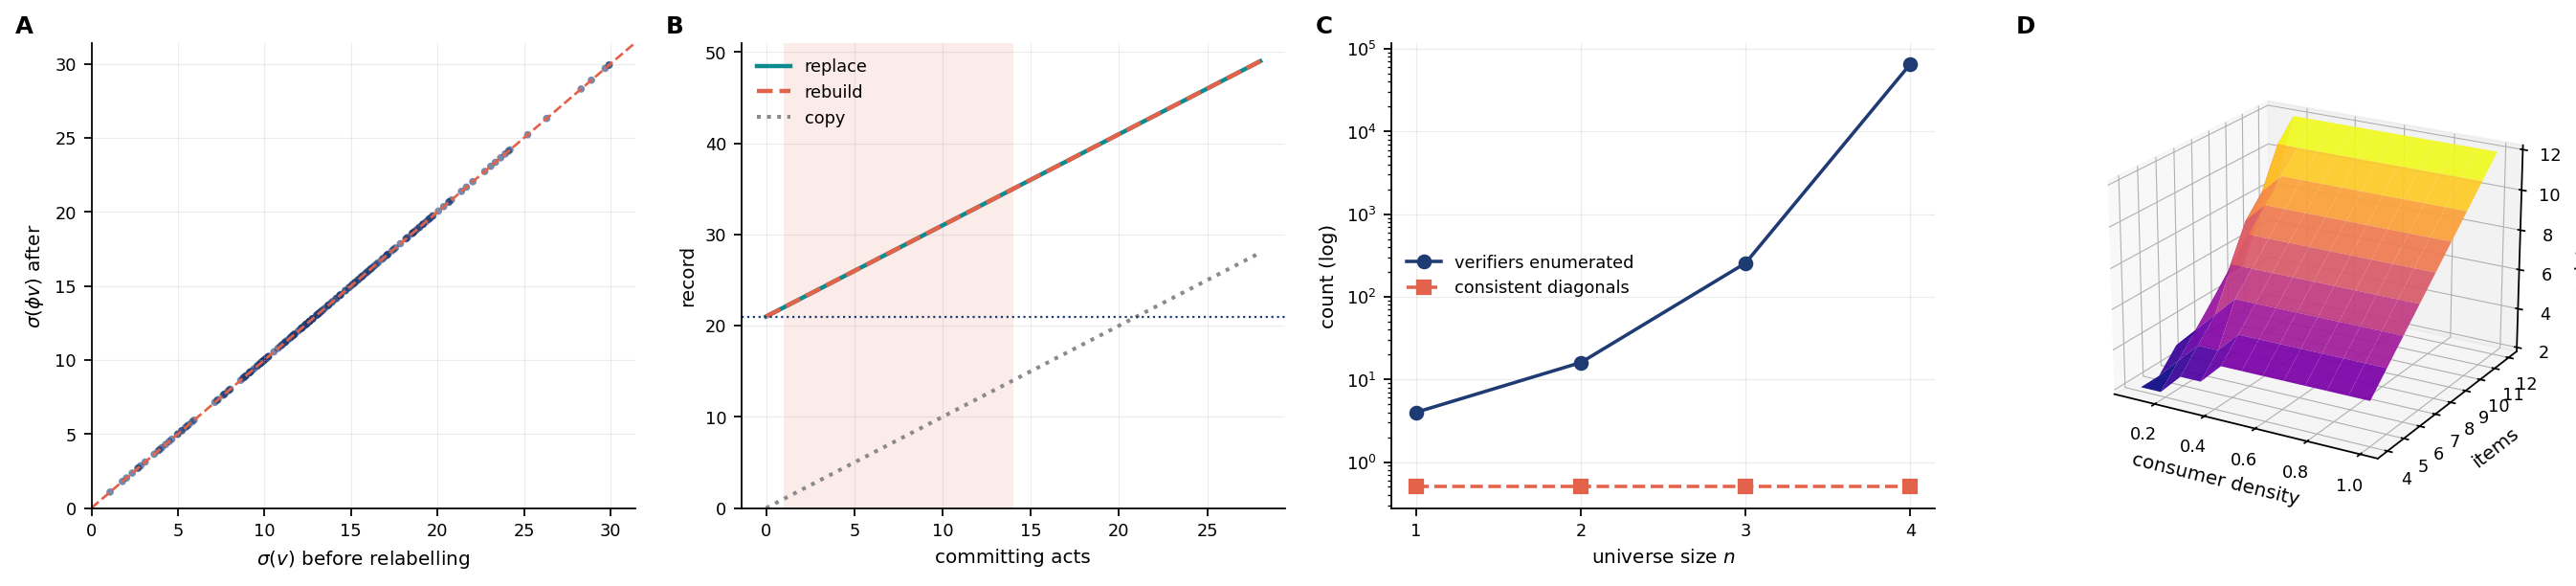
\includegraphics[width=\textwidth]{figures/panel_2_identity.png}
    \caption{\textbf{The Invariant Is Conserved; the Record and the
    Termination Condition Are What Separate Individuals.}
    (\textbf{A})~Separation cost after a random weighted relabelling on the
    linear $y$-axis versus the cost before on the linear $x$-axis, for all
    $423$ items of $60$ random graphs. Every point lies exactly on the identity
    diagonal (crimson dashed): the maximum discrepancy over the whole
    population is $0$, while $365$ of the $423$ labels were moved by the
    permutation. The datum the relabelling fixes and the datum it moves are
    plotted on the same instances---empirical content of
    Theorem~\ref{thm:invariant} (Conserved Invariant).
    (\textbf{B})~Record trajectories for the three cases of
    Theorem~\ref{thm:termination-crit} on a seven-plank structure: committed
    record on the linear $y$-axis versus committing acts on the linear
    $x$-axis. Gradual replacement (teal) and disassembly-then-reconstruction
    (crimson dashed) climb identically and share the same $\Char$; the shaded
    interval is the stage at which the reconstructed structure is \emph{open}
    in the sense of Definition~\ref{def:terminated}, which is what makes it a
    distinct individual. The copy (grey dotted) climbs on a separate lineage
    from zero. The navy reference is the record at which construction
    completed. $\Char$ is preserved in all three cases; only the record chain
    and the open stage discriminate.
    (\textbf{C})~The diagonal of Theorem~\ref{thm:self-diagonal}, enumerated
    exhaustively: total verifiers on a universe of size $n$ (navy, $2^{2^{n}}$,
    reaching $65{,}536$ at $n=4$) against the number admitting a consistent
    diagonal value (crimson squares), both on a log $y$-axis versus $n$ on the
    linear $x$-axis ($1$ to $4$). The crimson series is identically zero at
    every $n$; a single consistent case anywhere in the enumeration would
    falsify the theorem. This is a proof by exhaustion over the stated finite
    domain, not a sampled test.
    (\textbf{D})~The cell an item registers, as a three-dimensional surface
    (plasma) over consumer density on the $x$-axis ($0.1$ to $1.0$) and item
    count on the $y$-axis ($4$ to $12$), elevation $21^{\circ}$ azimuth
    $-60^{\circ}$. The same item registers a thin cell in a sparse consumer and
    a rich one in a dense consumer; across $40$ paired trials the registrations
    differed in every case and both attained their own graph's floor in every
    case. No registration is privileged---the geometry of
    Theorem~\ref{thm:receiver} (Consumer-Relativity).}
    \label{fig:panel2}
\end{figure*}


% =====================================================================
\section{The record, and why it cannot be undone}
\label{sec:record}
% =====================================================================

The invariant of \Cref{sec:identity} is static. We now make cuts dynamic and
derive the second half of the identity criterion.

\begin{definition}[Committed cut; process; record]
\label{def:committed}
A \emph{cut event} commits a contact $e\in\E$ as a realised separation. A
\emph{process} is a finite sequence $P=(e_1,\dots,e_k)$ of distinct
committing acts. The \emph{committed record} is $\rec(P)=k$. The
\emph{residue} of $e_i$ is $\res_i:=\wt(e_i)\ge\flo>0$ by \Cref{thm:floor}.
\end{definition}

\begin{theorem}[Residue is the causal propagator]
\label{thm:propagator}
In a process, the residue $\res_i>0$ of cut $e_i$ is necessary and sufficient
for $e_{i+1}$ to be a distinct committing event: $e_{i+1}$ is a new cut if and
only if the state after $e_i$ differs from the state before, which holds if
and only if $\res_i>0$.
\end{theorem}

\begin{proof}
$e_{i+1}$ is distinct exactly when it acts on a state changed by $e_i$. The
only change $e_i$ effects is depositing its residue $\res_i$. If $\res_i>0$
the post-state carries a committed contact absent before, so $e_{i+1}$ acts on
a strictly different configuration and is distinct. If $\res_i=0$---excluded
by \Cref{thm:floor}, and considered here only for the necessity
direction---pre- and post-states coincide and $e_{i+1}$ has no changed state
to act on. Hence $\res_i>0$ is necessary and sufficient.
\end{proof}

\begin{corollary}[A process is a residue chain]
\label{cor:chain}
A process is a chain in which each cut's residue causes the next:
$\res_1\to e_2$, $\res_2\to e_3$, and so on. Remove any $\res_i$ and the chain
halts at step $i$.
\end{corollary}

\begin{theorem}[Monotone non-return]
\label{thm:monotone}
The committed record is strictly increasing along any process, and no process
decreases it. A process revisiting a configuration does not return to a prior
state: the configuration recurs but the record has strictly grown, and the
two states are distinguished by the record.
\end{theorem}

\begin{proof}
Each cut event increments $\rec$ by one (\Cref{def:committed}). To decrease
$\rec$, a committed contact would have to be un-committed; but un-committing
is itself a further committing act---a new cut redrawing the boundary---which
increments $\rec$. Hence $\rec$ is monotone. Two states with equal
configuration but records $r<r'$ are separated by the partition ``record
$\le r$'' versus ``record $>r$,'' hence are distinct states: recurrence of
configuration is not return of state.
\end{proof}

\begin{corollary}[The record is an intrinsic order]
\label{cor:record-time}
\Cref{thm:monotone} attaches to every process a monotone scalar that never
decreases and that distinguishes equal configurations at different counts.
``Before'' and ``after'' are the order on the record; the order is intrinsic
to the sequence of cuts and requires no external parameter
\citep{lamport1978}.
\end{corollary}

\begin{theorem}[Three readings of a residue]
\label{thm:three}
A residue $\res_i$ admits exactly three readings, according to how its link to
the next cut is resolved:
\begin{enumerate}[label=\textup{(\roman*)},leftmargin=2.0em,itemsep=1pt]
\item \emph{order}---as the increment of the record (\Cref{thm:monotone});
\item \emph{information}---when tracked as the specific cause of a specific
next cut, a resolved link;
\item \emph{entropy}---when residues are present but their links are
untracked, their aggregate is the Shannon content $H=-\sum_i p_i\log p_i$ of
the unresolved-link distribution \citep{shannon1948,cover2006}.
\end{enumerate}
Tracking moves a process from entropy toward information; losing track moves
it back.
\end{theorem}

\begin{proof}
(i) is \Cref{thm:monotone}. (ii) a tracked link is a determinate map
$\res_i\mapsto e_{i+1}$; specifying it for each $i$ specifies the chain
exactly. (iii) with links unresolved, the chain is known only through the
distribution over which residue caused which next cut, whose information
content is $H$ \citep{shannon1948}. Resolving links converts an unknown
distribution into determinate functions.
\end{proof}

\begin{remark}[Why the three readings matter here]
\label{rem:three-matters}
\Cref{thm:three} is used twice below. In \Cref{sec:reification} it explains
precisely what is lost when a prior determination is re-presented as content
rather than retained as structure: the links are gone, so the information
reading degrades to the entropy reading. In \Cref{sec:construction} it
underwrites the discipline of carrying committed structure rather than
carrying the material from which the structure was drawn.
\end{remark}

% =====================================================================
\section{The self-blunting instrument}
\label{sec:cut}
% =====================================================================

We now prove the paper's first main result. It concerns not what is cut, but
what does the cutting.

\begin{definition}[Contact operation; instrument and sample]
\label{def:contact-op}
A \emph{contact operation} is a single cut event (\Cref{def:committed}): one
committed edge $\set{u,v}$, individuating two items by depositing residue
$\ge\flo$. Reading the operation with $u$ as the \emph{instrument} and $v$ as
the \emph{sample} is a choice of description; the operation itself is the
committed edge.
\end{definition}

\begin{theorem}[Symmetry of individuation]
\label{thm:symmetry}
A contact operation is symmetric in its endpoints. Committing $\set{u,v}$
commits a boundary edge of $u$ exactly as it commits a boundary edge of $v$:
$\set{u,v}\in\cut(\set{u})$ and $\set{u,v}\in\cut(\set{v})$, and the residue
deposited is the same weight $\wt(\set{u,v})\ge\flo$ on both readings. There
is no assignment of the operation to one endpoint that leaves the other
untouched.
\end{theorem}

\begin{proof}
By \Cref{def:graph} an edge is an unordered pair, and by \Cref{def:committed}
a cut event commits the edge, not an orientation of it. The edge lies in the
singleton cut of each endpoint by definition of $\cut(\cdot)$, and its weight
is a single number attached to the edge, not to an endpoint. So both
endpoints acquire a committed boundary edge of that weight, and neither
acquires it without the other.
\end{proof}

\begin{definition}[Edge capacity of an instrument]
\label{def:capacity}
The \emph{edge capacity} of a vertex $u$ at a given stage is the set of
contacts incident to $u$ that have not yet been committed. Its cardinality is
$\mathrm{cap}(u)$.
\end{definition}

\begin{theorem}[One use]
\label{thm:one-use}
A given cut---a given committed edge $e=\set{u,v}$---is committed exactly
once. Any later cut at $u$ or at $v$ is either a distinct edge, or the same
edge at a strictly higher record, hence a different cut event. There is no
re-commitment of the same cut.
\end{theorem}

\begin{proof}
Committing $e$ increments the record (\Cref{def:committed}). A second
``commitment'' of $e$ is either a no-op---the edge is already committed, so no
new cut event occurs and no residue is deposited---or a distinct event at
record $\rec+1$, which by \Cref{thm:monotone} is a different state and hence a
different cut event. In neither case is the original cut repeated.
\end{proof}

\begin{theorem}[Self-blunting]
\label{thm:blunt}
A contact operation changes the instrument. After committing $\set{u,v}$,
the instrument $u$ has strictly reduced edge capacity,
$\mathrm{cap}(u)$ decreasing by one, and strictly increased record. Both
changes are irreversible.
\end{theorem}

\begin{proof}
By \Cref{thm:symmetry} the operation commits a boundary edge of $u$ exactly as
of $v$. The committed edge leaves $u$'s uncommitted-contact set
(\Cref{def:capacity}), strictly reducing $\mathrm{cap}(u)$. The record
increases by \Cref{def:committed}. Irreversibility of the record is
\Cref{thm:monotone}; irreversibility of the capacity reduction follows,
since restoring the edge to the uncommitted set would be an un-commitment,
which \Cref{thm:monotone} shows is itself a further committing act rather
than a reversal. Hence the instrument after the operation differs from the
instrument before, in capacity and in record.
\end{proof}

\begin{theorem}[No perfect repeatable instrument]
\label{thm:no-perfect}
There is no contact operation that both
\begin{enumerate}[label=\textup{(\roman*)},leftmargin=2.0em,itemsep=1pt]
\item separates two items at zero residue (a \emph{traceless} operation), and
\item leaves the instrument unchanged (a \emph{repeatable} instrument).
\end{enumerate}
Property (i) requires $\flo=0$, forbidden by \Cref{thm:floor}; property (ii)
requires the record to be unchanged by a cut, forbidden by
\Cref{thm:monotone}. Each is separately impossible, so their conjunction is a
fortiori impossible.
\end{theorem}

\begin{proof}
(i): a traceless operation deposits residue $0$, i.e.\ commits an edge of
weight $0$, contradicting $\wt(e)\ge\flo>0$ (\Cref{thm:floor}). (ii): an
unchanged instrument requires the record after to equal the record before,
contradicting the strict increment of \Cref{def:committed} and
\Cref{thm:monotone}; and by \Cref{thm:blunt} the capacity strictly decreases
as well.
\end{proof}

\subsection{The stateless predictor occupies the forbidden position}
\label{sec:stateless}

We can now state the consequence for the object described in
\Cref{sec:intro}.

\begin{definition}[Stateless determiner]
\label{def:stateless}
A \emph{stateless determiner} is a map $D$ from queries to determinations
such that (a) $D$ is fixed by a prior procedure and is not altered by being
applied, and (b) applying $D$ commits no cut in the graph against which its
determinations are made. Its \emph{record} is constant across applications.
\end{definition}

\begin{corollary}[A stateless determiner claims the forbidden position]
\label{cor:stateless-forbidden}
A stateless determiner asserts, of each of its applications, both properties
of \Cref{thm:no-perfect}: the application deposits no residue into the
determiner (property (ii)), and---since a determination made without
committing a cut separates its answer from the medium at no cost---the
application is traceless (property (i)). No contact operation has either
property, so a stateless determiner's applications are not contact
operations, and its determinations are not individuations in the sense of
\Cref{def:sepcost}.
\end{corollary}

\begin{proof}
Property (ii) is \Cref{def:stateless}(a) together with the constancy of the
record: by \Cref{thm:blunt} every contact operation strictly reduces the
instrument's capacity and increments its record, and by hypothesis neither
occurs. Property (i) is \Cref{def:stateless}(b): a determination that commits
no edge deposits residue $0$, which by \Cref{cor:no-sharp} no individuation
does. Hence by \Cref{thm:no-perfect} the applications cannot be contact
operations, and by \Cref{def:sepcost} what they return is not the resting cut
of anything in the graph.
\end{proof}

\begin{remark}[What the corollary does and does not say]
\label{rem:corollary-honest}
\Cref{cor:stateless-forbidden} is not an empirical claim that trained
predictors are wrong, nor a claim that their outputs are useless. It is a
statement about \emph{type}: whatever a stateless determiner returns, it is
not an individuation of an item against a medium, because individuation is a
committed cut and no cut was committed. The output may be valuable, may be
correct, and may be exactly what a downstream consumer needs. What it lacks
is the trace that would make it accountable, and the deposit that would make
the determiner a participant in the structure it reports on.
\end{remark}

\subsection{Staleness and reification: two visible symptoms}
\label{sec:reification}

The structural fact of \Cref{cor:stateless-forbidden} has two observable
consequences, and we record them because they are the phenomena that
motivate the construction of \Cref{part:pair}.

\begin{proposition}[Staleness]
\label{prop:staleness}
Let $D$ be a determiner whose determinations were fixed at record $\rec_1$,
and suppose $D$ is applied at a later record $\rec_2>\rec_1$ in a system whose
graph has changed between the two. Then the determination $D$ returns at
$\rec_2$ is the determination appropriate to the graph as it stood at
$\rec_1$. Since by \Cref{thm:monotone} no operation returns the system to the
state at $\rec_1$, the returned determination is one the system at $\rec_2$
could not now re-derive.
\end{proposition}

\begin{proof}
$D$'s determinations are fixed at $\rec_1$ by hypothesis, so each is the
terminus of whatever individuation the graph at $\rec_1$ supported. Every
committed cut between $\rec_1$ and $\rec_2$ altered the graph
(\Cref{thm:propagator}); by \Cref{thm:monotone} the record cannot be lowered
and the earlier configuration is not re-occupied as a state. Hence the
determination corresponds to a state the system has irreversibly left, and a
fresh individuation at $\rec_2$ need not return it.
\end{proof}

\begin{proposition}[Reification]
\label{prop:reification}
Let a prior propagation $P=(e_1,\dots,e_k)$ be re-presented to a determiner
as content---that is, as a description supplied among its inputs rather than
as committed structure in the graph. Then:
\begin{enumerate}[label=\textup{(\roman*)},leftmargin=2.0em,itemsep=1pt]
\item the re-presentation does not restore the state at which $P$ was
committed (\Cref{thm:monotone});
\item the links of $P$---which residue caused which next cut---are not
recoverable from the description, so $P$ enters under the entropy reading of
\Cref{thm:three}(iii) rather than the information reading
\Cref{thm:three}(ii);
\item consequently the determiner reasons about a degraded image of $P$, and
the act of doing so is itself a further event, so what is reasoned about is
not what $P$ was.
\end{enumerate}
\end{proposition}

\begin{proof}
(i) is \Cref{thm:monotone}: configuration may recur, state does not. (ii) A
description of $P$ lists its deposits; the causal links $\res_i\mapsto
e_{i+1}$ are not deposits but relations between successive states
(\Cref{thm:propagator}), and are not recoverable from a listing of the
deposits alone, since distinct link structures over the same deposits are
possible. By \Cref{thm:three} the unresolved-link reading is the entropy
reading. (iii) By \Cref{thm:monotone} the re-presentation occurs at a record
strictly greater than that at which $P$ was committed, so the object under
consideration---a description at the later record---is not the process $P$ at
the earlier one.
\end{proof}

\begin{remark}[The category change is the defect]
\label{rem:category-change}
\Cref{prop:reification} identifies something sharper than information loss.
A committed propagation is a \emph{cause}: its residue is what makes the next
cut possible (\Cref{thm:propagator}). Re-presented as content, it becomes an
\emph{object under inspection}. The two are different categories, and the
conversion is one-way: by \Cref{thm:three} the links that made it a cause are
exactly what the description does not carry. This is why, in the construction
of \Cref{part:pair}, prior propagation is retained as committed edges in the
graph and never re-supplied as material. There is then nothing to re-present,
because the propagation changed \emph{what the system is} rather than
producing a record for the system to read.
\end{remark}

\begin{figure*}[!htbp]
    \centering
    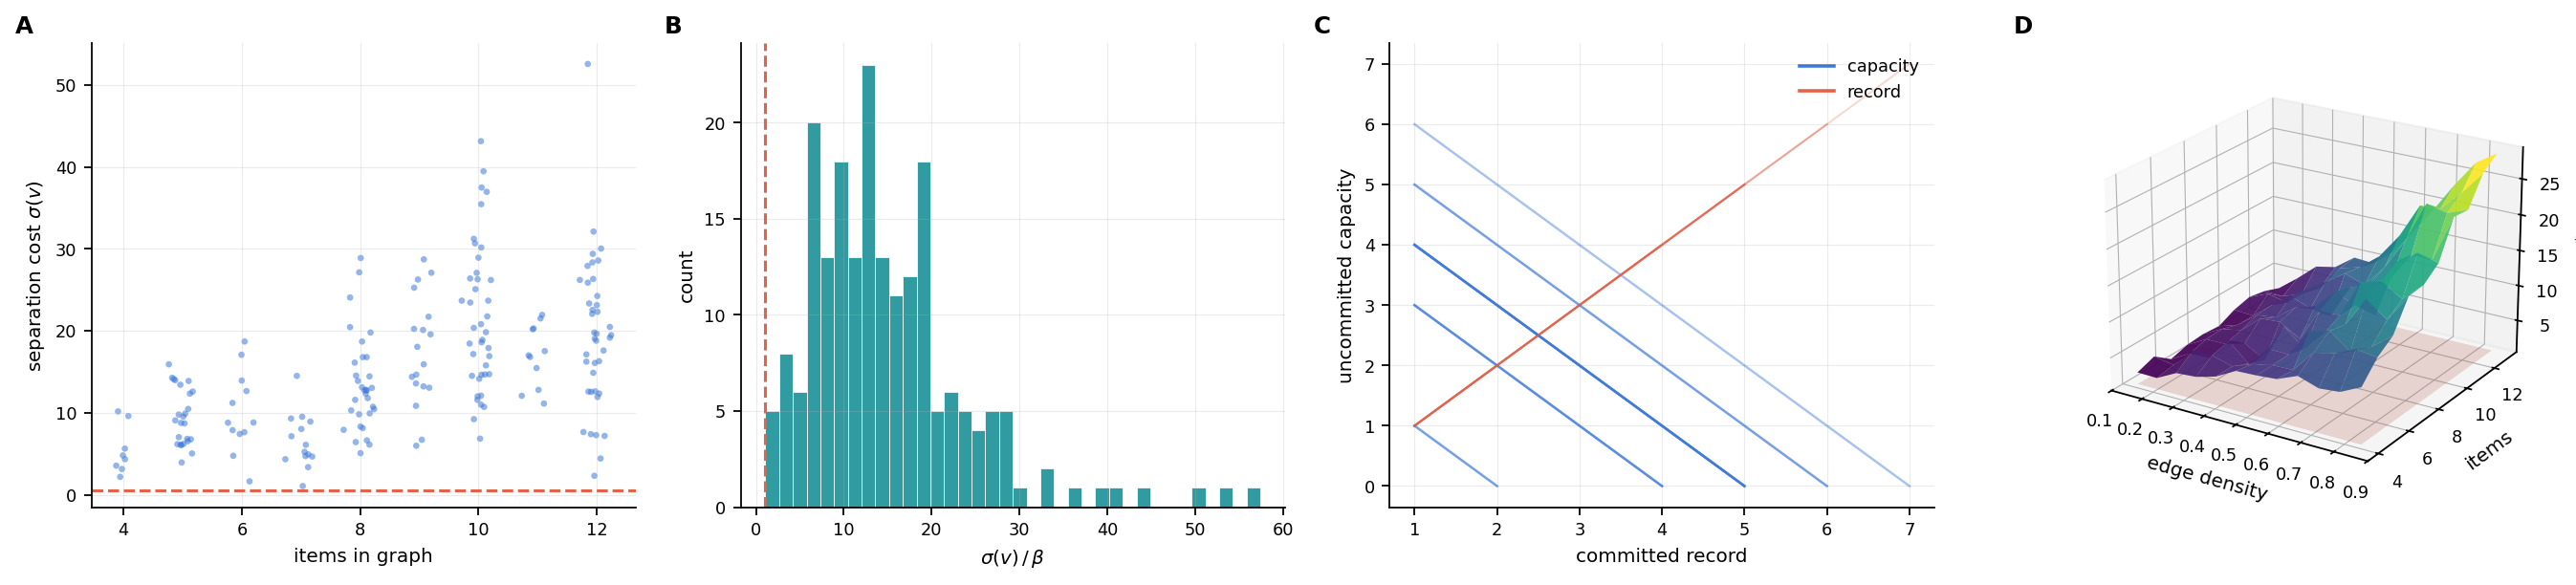
\includegraphics[width=\textwidth]{figures/panel_1_floor_blunting.png}
    \caption{\textbf{The Floor Is Positive and Every Act Consumes the
    Instrument.}
    (\textbf{A})~Separation cost $\str(v)$ on the linear $y$-axis versus the
    number of items in the graph on the linear $x$-axis ($4$ to $12$), for all
    $489$ realised separations drawn from $60$ random contact graphs at floors
    $\flo\in\{0.5,1.0,2.0\}$; points are jittered horizontally to separate
    graphs of equal size. The crimson dashed line is the floor. No point lies
    beneath it at any graph size---$0$ violations, minimum realised cost
    $0.600$---while the ceiling rises with graph size, since an item entangled
    with more others is more expensive to separate. Empirical content of
    Theorem~\ref{thm:floor} (Positive Floor).
    (\textbf{B})~Distribution of the normalised cost $\str(v)/\flo$ on the
    linear $x$-axis ($1$ to $57.4$), $36$ bins, over the same $489$
    separations. The support begins at and never crosses the crimson reference
    at $1$; the mass concentrated just above it is the population of items
    individuated by a single contact, the cheapest genuine separation, and the
    long right tail is the population individuated only by triangulating many
    weak contacts.
    (\textbf{C})~The self-blunting trajectories of Theorem~\ref{thm:blunt} for
    fourteen instruments: uncommitted capacity on the linear $y$-axis versus
    committed record on the linear $x$-axis. Capacity (steel) falls by exactly
    one and the record (crimson) rises by exactly one at every contact
    operation, the two crossing as capacity is spent. All $30$ tested
    instruments are strictly blunted and all $30$ exhibit the crossing; none
    escapes either movement.
    (\textbf{D})~Realised system floor $\flo^{\ast}$ as a three-dimensional
    surface (viridis) over edge density on the $x$-axis ($0.15$ to $0.85$) and
    item count on the $y$-axis ($4$ to $13$), each cell the mean of six random
    graphs, viewing angle elevation $22^{\circ}$ azimuth $-58^{\circ}$. The
    translucent crimson plane beneath is $\flo=1$. The surface lies above the
    plane at every density and every size, rising with both: the floor is a
    trace the non-completable medium leaves on every finite part
    (Remark~\ref{rem:floor-fact}), not an artefact of a particular graph.}
    \label{fig:panel1}
\end{figure*}

% =====================================================================
\section{What a structure cannot know about itself}
\label{sec:unknowability}
% =====================================================================

Two independent arguments place the invariant of \Cref{sec:identity} out of
reach of the structure that carries it. We need both, because they have
different hypotheses and different strengths.

\begin{theorem}[The invariant is not extractable as a value]
\label{thm:unextractable}
There is no operation that reads the resting cut of an item off as a
residue-free value. Such a reading would require $\res(v)=0$, which by
\Cref{thm:floor-derived} requires the whole to be brought to bear---i.e.\
requires the reader to occupy the item's entire negation structure, which by
\Cref{cor:nonneighbours} is what individuates the item. An operation
occupying both sides of the constituting partition is not a comparison.
\end{theorem}

\begin{proof}
By \Cref{thm:region} the invariant is a cut of weight $\ge\flo$; reducing it
to a point is $\res(v)=0$, excluded by \Cref{thm:floor-derived}. Concretely,
to fix $v$ exactly is to decide it against the totality of what it is not
(\Cref{thm:negation}); a reader performing that decision is itself within
that totality, so a complete reading would require it to be simultaneously
the part read and the whole the part is read against. The gap that keeps the
two apart is exactly the residue $\ge\flo$.
\end{proof}

\begin{definition}[Verifier; self-verification]
\label{def:verifier}
A \emph{verifier} is a map $\mathsf{V}$ that, given a part $X$ and a
candidate constituting totality $T$, returns $\mathsf{V}(X,T)\in\set{0,1}$,
reading $1$ exactly when $X$ is the part $T$ constitutes, i.e.\ when
$X=\V\setminus T$. To \emph{self-verify} is to evaluate $\mathsf{V}$ on the
part its own verdicts constitute---its own negation.
\end{definition}

\begin{theorem}[No consistent self-verification]
\label{thm:self-diagonal}
Let $D:=\set{X:\mathsf{V}(X,\co X)=0}$. If $\mathsf{V}$ is total---returning a
value on every part and its negation---and $D$ is itself a part on which
$\mathsf{V}(\cdot,\co\,\cdot)$ is defined, then $\mathsf{V}(D,\co D)$ has no
consistent value: each of the two possible values entails the other.
\end{theorem}

\begin{proof}
Suppose $\mathsf{V}(D,\co D)=1$. Then $D$ is declared constituted by $\co D$;
but membership in $D$ is the condition $\mathsf{V}(X,\co X)=0$, so $D$'s
satisfying its own membership condition forces $\mathsf{V}(D,\co D)=0$.
Suppose instead $\mathsf{V}(D,\co D)=0$. Then $D$ meets its own membership
condition, hence is among the parts $D$ collects, which is the assertion
$\mathsf{V}(D,\co D)=1$. Both values are self-refuting; neither is consistent.
The argument is the diagonal of \citet{cantor1891}, in the undecidability
shape of \citet{godel1931,tarski1936,turing1936} and the fixed-point form of
\citet{lawvere1969}.
\end{proof}

\begin{remark}[The strength of each argument]
\label{rem:two-arguments}
\Cref{thm:self-diagonal} is exactly as strong as its closure
hypothesis---that the behaviour-defined $D$ is again a part on which
$\mathsf{V}$ acts. A verifier that is itself part of the graph it ranges over
makes the hypothesis natural, since its verdicts leave traces in the same
whole. We do not claim to discharge it in general. We mark it, and note that
\Cref{thm:unextractable}---the floor argument---holds without it. What rides
on the closure hypothesis is only the sharper claim that self-verification is
forbidden \emph{directly} rather than merely unattainable.
\end{remark}

\begin{definition}[Consumer; registered cell]
\label{def:consumer}
A \emph{consumer} is a contact graph, understood as a system that
individuates items against its own rest. The \emph{cell an item registers}
in a consumer is the item's resting cut computed in that consumer's graph.
\end{definition}

\begin{theorem}[Consumer-relativity: distinct consumers register distinct
cells, each correct]
\label{thm:receiver}
The same item registers different cells in consumers with different graphs,
and each registration is a correct individuation at that consumer's floor. No
registration is privileged as ``the'' identity, and there is no point-valued
identity of which the registrations are approximations.
\end{theorem}

\begin{proof}
By \Cref{def:consumer} the registered cell is the item's resting cut in the
consumer's graph; different graphs yield different cuts---a sparse graph
individuates the item against few contrasts, giving a thin cell; a dense one
against many, giving a rich cell. Each is the minimum-cut individuation in
its own graph and hence correct there, attaining that graph's floor by
\Cref{thm:floor}. Were there a privileged point-valued identity, a
registration differing from it would be incorrect; but each registration is
correct in its own graph, and by \Cref{thm:unextractable} no point-valued
identity exists to be approximated. Hence none is privileged.
\end{proof}

\begin{theorem}[No runtime verdict]
\label{thm:no-verdict}
A system whose vocabulary over its graph consists of identifying an item,
reading its committed values, transforming internally, and committing new
values, cannot issue a verdict of success or failure on a determination.
\end{theorem}

\begin{proof}
A verdict is a comparison of an achieved state to an expected one. The stated
vocabulary contains no term for an expectation: the graph stores what was
committed (\Cref{def:committed}), not what should have been committed, and by
\Cref{thm:receiver} there is no privileged registration against which an
achieved cell could be measured. The system therefore holds no expected state
and possesses no comparison operator, so there is no quantity it could
compute having the meaning of a verdict. Adjudication is possible only in a
consumer holding an expectation of its own, and such a judgement is that
consumer's, not the system's.
\end{proof}

\begin{remark}[Why this is a feature of the design]
\label{rem:no-verdict-feature}
\Cref{thm:no-verdict} is the formal content of a runtime that runs to
completion and records anomalies rather than raising them. An unexpected
determination is committed as a value like any other and is available to any
consumer that reads it. What is refused is not error handling but the
runtime's arrogation of a judgement that \Cref{thm:receiver} shows belongs to
consumers. \Cref{sec:closure} supplies the honest terminal states such a
system \emph{can} report.
\end{remark}

% =====================================================================
\section{The identity criterion}
\label{sec:identity-criterion}
% =====================================================================

We now assemble \Cref{sec:identity} and \Cref{sec:record} into a criterion,
and test it against the classical puzzles of persistence through change
\citep{plutarch,lewis1976,wiggins2001}.

\subsection{Neither component suffices alone}

\begin{proposition}[$\Char$ alone is not an identity criterion]
\label{prop:char-insufficient}
There exist contact graphs $\Gph$ and $\Gph'$ with $\Char(\Gph)=\Char(\Gph')$
that are not the same individual under any reasonable criterion: take
$\Gph'$ a faithful reconstruction of $\Gph$ built independently, or a copy of
$\Gph$ authored alongside it.
\end{proposition}

\begin{proof}
$\Char$ is a weighted-graph invariant (\Cref{prop:char}), so any $\Gph'$
isomorphic to $\Gph$ has $\Char(\Gph')=\Char(\Gph)$. Isomorphic graphs
include reconstructions and copies. Since a copy is uncontroversially a
distinct individual from its original---they may be operated on
independently, and a change to one does not change the other---$\Char$ does
not discriminate individuals.
\end{proof}

\begin{proposition}[$\rec$ alone is not an identity criterion]
\label{prop:rec-insufficient}
The record is a non-negative integer carrying no information about what is
being counted; two unrelated structures may stand at equal records.
\end{proposition}

\begin{proof}
Immediate from \Cref{def:committed}: $\rec$ counts committing acts and is
determined by their number alone.
\end{proof}

\begin{definition}[Individual]
\label{def:individual}
An \emph{individual} is the pair $(\Char,\rec)$ carried by a structure: its
conserved invariant together with its committed record. Two structures are
\emph{the same individual} at two moments if and only if there is a chain of
committing acts joining them along which $\Char$ is preserved and $\rec$ is
strictly increasing, with no intervening stage at which any unit of the
structure fails to be terminated in the sense of \Cref{def:terminated}.
\end{definition}

\subsection{Termination is the operative criterion}

\begin{definition}[Terminated and open units]
\label{def:terminated}
A \emph{unit} is a connected item set $U$ with its induced contact structure.
It is \emph{terminated} if its resting cut against the medium is attained,
giving a definite separation cost $\str(U)\ge\flo$; it is \emph{open} if no
such cut is attained.
\end{definition}

\begin{theorem}[Only terminated units are individuated]
\label{thm:terminate}
A unit has a defined separation cost, hence a defined identity in the sense
of \Cref{thm:region}, only if terminated. An open unit has no attained cut
against the medium and therefore no defined identity.
\end{theorem}

\begin{proof}
Identity is the resting cut (\Cref{thm:region}), which by \Cref{def:sepcost}
is the attained minimiser of the separation cost. If no such cut is attained,
the quantity is undefined and no invariant is assigned.
\end{proof}

\begin{remark}[Termination is not free]
\label{rem:termination-cost}
Committing a completion boundary---making a collection of parts into a
definite unit---is itself a cut and deposits residue $\ge\flo$
(\Cref{cor:no-sharp}). The act of making a thing a definite thing already
pays the floor. This is what makes \Cref{thm:termination-crit} below
non-trivial.
\end{remark}

\begin{theorem}[Continuity of termination, not of parts]
\label{thm:termination-crit}
Let a structure undergo a sequence of committing acts.
\begin{enumerate}[label=\textup{(\roman*)},leftmargin=2.0em,itemsep=2pt]
\item \emph{Gradual replacement.} If parts are replaced one at a time in such
a way that the unit is terminated at every intermediate stage, then $\Char$ is
preserved, $\rec$ increases continuously, and the individual persists---even
if every part is eventually replaced.
\item \emph{Disassembly and reconstruction.} If the structure is fully
disassembled and then reassembled to identical specification, the resulting
structure has $\Char$ equal to the original but is a distinct individual.
\item \emph{Copying.} A structure authored alongside an original, to identical
specification, is a distinct individual regardless of $\Char$.
\end{enumerate}
\end{theorem}

\begin{proof}
(i) Each replacement is a committing act on a terminated unit; by
\Cref{thm:invariant} the invariant is preserved under any re-encoding
preserving the cut structure, and replacing a part while preserving the
contacts and weights is such a re-encoding. By \Cref{thm:monotone} the record
strictly increases at each act, and by hypothesis no stage leaves the unit
open, so \Cref{def:individual} is satisfied along the chain. That the parts
are eventually wholly replaced is irrelevant: by \Cref{thm:region} the
identity is borne by the cut structure, not by any vertex.

(ii) Disassembly leaves the unit open (\Cref{def:terminated}): no resting cut
is attained, so by \Cref{thm:terminate} no invariant is assigned at that
stage. \Cref{def:individual} requires that no intervening stage be open,
which fails. Equality of $\Char$ after reassembly follows from
\Cref{thm:invariant}, since the reassembled structure is isomorphic to the
original; but reassembly is a fresh termination, paying the floor again
(\Cref{rem:termination-cost}) and committing new cuts at strictly higher
record. By \Cref{thm:monotone} the record cannot be restored to its
pre-disassembly value, so the reassembled structure stands at a record whose
chain to the original passes through an open stage. Hence it is a distinct
individual.

(iii) A copy is isomorphic, so $\Char$ agrees by \Cref{thm:invariant}. But no
chain of committing acts joins the two: the copy's record was advanced by its
own authoring acts, not by acts on the original, and by \Cref{thm:monotone}
neither record is a continuation of the other. \Cref{def:individual} fails.
\end{proof}

\begin{table}[t]
\centering\small
\caption{The identity criterion adjudicating the classical cases. $\Char$ is
preserved in all three; the record and the termination condition separate
them.}
\label{tab:theseus}
\begin{tabular}{@{}lccc@{}}
\toprule
\textbf{Case} & $\Char$ & \textbf{record} & \textbf{same individual?}\\
\midrule
parts replaced singly   & preserved & continuous chain & \textbf{yes}\\
disassembled, rebuilt   & preserved & chain via open stage & \textbf{no}\\
copy authored alongside & identical & separate lineage & \textbf{no}\\
\bottomrule
\end{tabular}
\end{table}

\begin{corollary}[Snapshot and restore does not preserve an individual]
\label{cor:snapshot}
Serialising a structure and later reconstructing it from the serialisation
produces a structure with the same $\Char$ and a distinct individual.
\end{corollary}

\begin{proof}
Serialisation followed by reconstruction is disassembly followed by
reassembly to specification, which is \Cref{thm:termination-crit}(ii): the
serialised form is not a terminated unit in the graph---no resting cut of the
structure is attained while it is a byte string---so the chain passes through
an open stage.
\end{proof}

\begin{corollary}[Accretion is the only identity-preserving update]
\label{cor:accretion}
An update that adds items, contacts, and committed values to a structure
while leaving every unit terminated preserves the individual. An update that
tears down and rebuilds does not, however faithful the rebuild.
\end{corollary}

\begin{proof}
The first is \Cref{thm:termination-crit}(i); the second is
\Cref{thm:termination-crit}(ii).
\end{proof}

\begin{remark}[Engineering consequences]
\label{rem:engineering-identity}
\Cref{cor:snapshot,cor:accretion} are the two practical commitments the
criterion imposes on any system built on this account. Continuity across
restarts must be obtained by persisting the \emph{record} and accreting onto
it, never by reloading a serialised state as though it were the same
structure. Schema and content migrations must be performed accretively; a
rebuild is a replacement, not a refactor. Both are checkable predicates, not
matters of taste: the first asks whether the record is continuous, the second
whether any unit was left open.
\end{remark}

% =====================================================================
\part{The Causal Propagation Table}
\label{part:table}
% =====================================================================

% =====================================================================
\section{Alignment, accountability, and propagation}
\label{sec:table}
% =====================================================================

Part I fixed items at rest. We now make determination dynamic and construct
the object whose two evaluation regimes are the subject of the paper.

\subsection{Alignment}

\begin{definition}[Alignment; alignment score]
\label{def:alignment}
Fix a contact graph and a target item $x^{\star}$. The \emph{alignment} of an
item $x$ to $x^{\star}$ is the minimum-cut weight separating them,
\[
\str(x,x^{\star})\;=\;\min_{S\ni x,\ x^{\star}\notin S}\wt(\cut(S))\;\in\;[\flo,\Om],
\qquad \Om:=\wt(\E),
\]
and the \emph{alignment score} is $\al(x,x^{\star}):=\str(x,x^{\star})/\Om\in(0,1]$.
\end{definition}

\begin{lemma}[The floor bounds alignment below]
\label{lem:align-floor}
For distinct items $x\neq x^{\star}$, $\al(x,x^{\star})\ge\flo/\Om>0$: no two
distinct items are perfectly aligned.
\end{lemma}

\begin{proof}
Immediate from \Cref{thm:floor}: any $x$--$x^{\star}$ cut has weight $\ge\flo$,
and cuts are non-empty by connectivity.
\end{proof}

\begin{remark}[Uncertainty without an imported calculus]
\label{rem:no-prior}
The quantity ordinarily carried by a probability, a fuzzy membership, or a
posterior---a number in $[0,1]$ recording how sure---is carried throughout
this paper by $\al(\cdot,\cdot)$ and its distance to the floor $\flo/\Om$.
This quantity is derived (an exact minimum-cut weight), bounded below by
$\flo/\Om>0$, and parameter-free: no prior is set and no membership function
is tuned. Where a standard calculus \emph{posits} an uncertainty, the floor
\emph{forces} one. No theorem depends on the comparison.
\end{remark}

\subsection{The residual, accountability, and the floor of a system}

\begin{definition}[System floor]
\label{def:system-floor}
The \emph{system floor} of a contact graph is
$\flo^{\ast}:=\min_{v\in\V\setminus\set{\med}}\str(v)$, the least separation
cost of any item against the medium.
\end{definition}

\begin{definition}[Accountability]
\label{def:accountable}
Fix a tolerance $\eps\ge0$. A determination of $x^{\star}$ from $v_0$ is
\emph{$\eps$-accountable} when
\begin{equation}
\str(v_0,x^{\star})\;\le\;\flo^{\ast}\;+\;\eps\,\Om.
\label{eq:accountable}
\end{equation}
The \emph{accountable class} $\acc(v_0,x^{\star},\Proc)$ is the set of
propagations under $\Proc$ (\Cref{def:process}) from $v_0$ to $x^{\star}$
satisfying \eqref{eq:accountable}; it may be empty.
\end{definition}

\begin{remark}[Two independently movable quantities]
\label{rem:two-quantities}
The left side of \eqref{eq:accountable} is local to the queried pair: a single
minimum cut between $v_0$ and $x^{\star}$. The right side, at $\eps=0$, is a
minimum over \emph{every} item in the system, including items lying on no
path between the two. The whole of \Cref{sec:separation} is the observation
that these two can be moved independently and that no stored assertion
records either.
\end{remark}

\subsection{Processes and propagations}

\begin{definition}[Process graph; propagation]
\label{def:process}
A \emph{process graph} is a contact graph $\Proc=(\V,\E,\wt;\,I,x^{\star})$
together with a set $I\subseteq\V$ of \emph{seeds} and a designated
\emph{target} $x^{\star}\in\V$. A \emph{propagation} of a seed $v_0\in I$
through $\Proc$ is a walk $\Walk=(v_0,e_1,v_1,\dots,e_k,v_k)$ along edges of
$\Proc$ with $v_k=x^{\star}$; each edge $e_i$ is a contact operation
(\Cref{def:contact-op}). The \emph{trivial} or \emph{rest} process
$\Proc_{\mathrm{rest}}(v)$ has $I=\set{v}$, $x^{\star}=v$, and the single
available operation $\set{v,\med}$.
\end{definition}

\begin{theorem}[Convergence admissibility]
\label{thm:admissibility}
A propagation is \emph{admissible} if and only if it is convergent: its
terminal item is $x^{\star}$. Interior items are entirely unconstrained---an
interior item may have arbitrarily large alignment to the target, i.e.\ may be
maximally unlike it, without rendering the propagation inadmissible.
Inadmissibility arises exclusively from failure to reach $x^{\star}$, never
from local misalignment along the way.
\end{theorem}

\begin{proof}
By \Cref{def:process} a propagation terminates at $x^{\star}$ by construction,
and its terminal alignment is $\al(x^{\star},x^{\star})$, the least value
permitted by \Cref{lem:align-floor}; so every propagation in the defined sense
is convergent. A walk failing to reach $x^{\star}$ has terminal item
$v_k\neq x^{\star}$ and is not a propagation to $x^{\star}$; it is
inadmissible as a determination of $x^{\star}$. Nothing in \Cref{def:process}
constrains the alignment of any interior item: the walk is defined purely by
adjacency and by its terminus. Hence admissibility depends exclusively on the
terminal condition.
\end{proof}

\begin{theorem}[Path opacity]
\label{thm:path-opacity}
Let $\Walk_1,\Walk_2$ be two propagations of the same seed to the same target,
differing in their interior items. Then no invariant computed from the seed
and target alone---the seed, the target, the terminal alignment, or the
target's resting cut---distinguishes $\Walk_1$ from $\Walk_2$. The interior of
a propagation is unobservable from its result.
\end{theorem}

\begin{proof}
Every listed invariant is a function of the endpoints alone, hence identical
on the two propagations by hypothesis. The interior data are, by
\Cref{thm:admissibility}, unconstrained given the endpoints, so they are not
recoverable as a function of the endpoints; an invariant computed only from
the endpoints therefore cannot distinguish them.
\end{proof}

\begin{corollary}[The deliverable is a class, not a path]
\label{cor:gauge}
For fixed seed, target, and process, the admissible propagations form an
equivalence class under ``shares seed and target, and converges,'' every
member of which is indistinguishable from every other by any test of the
result alone. A determination's deliverable is properly this class.
\end{corollary}

\begin{proof}
Immediate from \Cref{thm:admissibility,thm:path-opacity}.
\end{proof}

\begin{remark}[Path opacity is not a limitation]
\label{rem:opacity-feature}
\Cref{thm:path-opacity} says the interior is not recoverable \emph{from the
result}. It does not say the interior is lost: the committed edges of
$\Walk_1$ and $\Walk_2$ differ in the graph, so the two propagations leave
different structures behind even though their outputs agree. This is the
distinction that \Cref{sec:reification} turns on. History is retained as
committed structure, and is precisely not retained as material available for
re-presentation---which is why \Cref{prop:reification} does not apply to a
system built this way.
\end{remark}

\subsection{Representation mobility}

\begin{definition}[Representation; representation fibre]
\label{def:representation}
Fix an item $v$ and a target $x^{\star}$, and write $\al=\al(v,x^{\star})$. A
\emph{representation} of $v$ at dimension $N$ is a tuple
$(s_1,\dots,s_N)\in\R^{N}$ satisfying the \emph{averaging constraint}
$\frac1N\sum_j s_j=\al$, with individual components otherwise unconstrained
in $\R$---in particular, a component may lie outside $(0,1]$. The
\emph{representation fibre} of $v$ at dimension $N$ is the set of all such
tuples.
\end{definition}

\begin{theorem}[Representation mobility]
\label{thm:rep-mobility}
For every item $v$ and every $N\ge2$:
\begin{enumerate}[label=\textup{(\roman*)},leftmargin=2.0em,itemsep=1pt]
\item the representation fibre is non-empty and infinite;
\item switching from one representation to another commits no new contact and
leaves the record unchanged;
\item any computation depending on $v$ only through $\al(v,x^{\star})$ is
invariant under representation switching.
\end{enumerate}
\end{theorem}

\begin{proof}
(i) The averaging constraint is a single linear equation in $N$ unknowns;
for $N\ge2$ its solution set is an affine hyperplane of $\R^{N}$, hence
non-empty and infinite, and any $(s_1,\dots,s_{N-1})$ extends uniquely by
$s_N=N\al-\sum_{j<N}s_j$. (ii) A switch replaces one tuple in the fibre with
another; both denote the same item at the same alignment, so the switch
introduces no new item, no new contact, and hence no committing act. (iii) By
hypothesis the computation is a function of $\al$ alone, and every fibre
member averages to the same value.
\end{proof}

\begin{remark}[Components may be individually inadmissible]
\label{rem:virtual-components}
\Cref{def:representation} deliberately permits components outside the range
that any single admissible item could occupy: only the \emph{mean} is
constrained. This is not a loophole but the substance of the definition. It
permits intermediate decompositions that are individually impossible while
their aggregate is exactly the required alignment---and by
\Cref{thm:rep-mobility}(iii) nothing downstream can tell the difference, since
downstream computations see only the mean. \Cref{thm:admissibility} is the
dynamic counterpart: interior steps of a propagation are unconstrained
provided the walk converges.
\end{remark}

\subsection{The table}

\begin{definition}[Causal propagation table]
\label{def:table}
The \emph{causal propagation table} of a contact graph is the map
\[
\Tab(v_0,x^{\star},\Proc)\;:=\;
\begin{cases}
\cut\bigl(S^{\ast}(x^{\star})\bigr) & \text{if }\acc(v_0,x^{\star},\Proc)\neq\varnothing,\\[2pt]
\varnothing & \text{otherwise,}
\end{cases}
\]
returning, for a seed, a target, and a process, the accountable terminal cut
of the propagation---or the verdict that no propagation from $v_0$ to
$x^{\star}$ under $\Proc$ is accountable.
\end{definition}

\begin{proposition}[The table's outputs are cuts of weight $\ge\flo$]
\label{prop:table-type}
Every non-empty output of $\Tab$ is a cut of weight $\ge\flo$ in the sense of
\Cref{def:sepcost}, hence an object of the same type as the resting cut of an
item.
\end{proposition}

\begin{proof}
By \Cref{def:table} a non-empty output is the resting cut of $x^{\star}$,
which by \Cref{thm:floor} has weight $\ge\flo$.
\end{proof}

\begin{proposition}[Edges are products of a run]
\label{prop:no-edges}
The causal relation on items is not a fixed attribute of the graph. A causal
edge $u\to v$ obtains in a propagation exactly when, in that propagation, a
value committed at $u$ was read at $v$. Consequently the causal edge set is a
product of a propagation, not an input to it, and two propagations over the
same item set may induce different causal edge sets.
\end{proposition}

\begin{proof}
By \Cref{def:committed} an edge becomes committed only by a cut event, and by
\Cref{def:process} which cut events occur is determined by the walk taken.
Two walks with different interiors---admissible by
\Cref{thm:admissibility}---commit different edges.
\end{proof}

% =====================================================================
\part{The Directional Pair}
\label{part:pair}
% =====================================================================

% =====================================================================
\section{The catalogue is the table at rest}
\label{sec:directional}
% =====================================================================

We now prove the paper's central theorem. It says that a catalogue of items
at rest and a machinery of propagation under process are not two objects but
one object at two settings of a single argument.

\subsection{The resting catalogue}

\begin{definition}[Resting catalogue]
\label{def:catalogue}
The \emph{resting catalogue} of a contact graph is the assignment, to each
item $v$, of its resting cut against the medium,
\[
\cell(v)\;:=\;\cut\bigl(S^{\ast}(v)\bigr),\qquad \str(v)\ge\flo.
\]
A catalogue \emph{cell} is the name of this cut: the invariant region by
which $v$ is told from the rest, at rest (\Cref{thm:region}).
\end{definition}

\begin{theorem}[A catalogue cell is an accountable output]
\label{thm:cell-is-output}
For each item $v$, the cell $\cell(v)$ equals the output of the table run on
$v$ against the medium under the trivial process:
\[
\cell(v)\;=\;\Tab\bigl(v,\;v,\;\Proc_{\mathrm{rest}}(v)\bigr).
\]
Equivalently, a catalogue entry is the convergent terminal cut of the resting
propagation.
\end{theorem}

\begin{proof}
Take $\Proc_{\mathrm{rest}}(v)$ as in \Cref{def:process}: seeds
$I=\set{v}$, target $x^{\star}=v$, and the single available contact
$\set{v,\med}$. The propagation is the one cut event individuating $v$ from
$\med$; it is admissible by \Cref{thm:admissibility} since it terminates at
its target, and its terminal accountable object is by \Cref{def:table} the
resting cut $\cut(S^{\ast}(v))$. This is precisely $\cell(v)$ by
\Cref{def:catalogue}. Accountability at the target is immediate: taking
$v_0=x^{\star}=v$ gives $\str(v,v)$ realised by the minimum cut against the
medium, and by \Cref{def:system-floor} this is $\ge\flo^{\ast}$ with equality
attained at the item realising the system floor, so
\eqref{eq:accountable} is satisfiable at $\eps=0$ and satisfied for all
$\eps\ge0$ at the realising item.
\end{proof}

\begin{theorem}[Directional identity: the catalogue is the table at rest;
the table is the catalogue propagated]
\label{thm:catalogue-table}
The resting catalogue is the restriction of the causal propagation table to
trivial processes:
\[
\cell(v)\;=\;\Tab\bigl(v,\,v,\,\Proc_{\mathrm{rest}}(v)\bigr)
\qquad\text{for every item }v .
\]
Conversely, for a nontrivial process $\Proc$ the output
$\Tab(v_0,x^{\star},\Proc)$ is an object of the \emph{same type} as a
catalogue cell---an accountable cut of weight $\ge\flo$, the convergent
terminal individuation of the tracked item---computed under propagation
rather than at rest.
\end{theorem}

\begin{proof}
The forward direction is \Cref{thm:cell-is-output}. For the converse: by
\Cref{thm:admissibility} every admissible propagation terminates at
$x^{\star}$, whose individuating datum is the resting cut
$\cut(S^{\ast}(x^{\star}))$ of weight $\ge\flo$ by \Cref{thm:floor}; by
\Cref{prop:table-type} this is the same type of object as $\cell(\cdot)$ in
\Cref{def:catalogue}. The two differ only in that the cut is the terminus of a
nontrivial propagation rather than of the rest contact. Hence the table's
output for a process is a catalogue-grade cut computed under propagation.
\end{proof}

\begin{corollary}[One object, two directions]
\label{cor:one-object}
A catalogue and a propagation machinery are not two systems requiring an
interface. They are one map $\Tab$ evaluated at two settings of its process
argument, whose outputs inhabit a single type. No translation between them is
required or possible: there is nothing to translate.
\end{corollary}

\begin{proof}
Immediate from \Cref{thm:catalogue-table}: both regimes are values of the same
map, and by \Cref{prop:table-type} both outputs are cuts of weight $\ge\flo$.
\end{proof}

\begin{remark}[The canonical instance]
\label{rem:periodic}
The familiar catalogue of chemical elements
\citep{mendeleev1869,scerri2007} is, on this reading, a resting catalogue in
the sense of \Cref{def:catalogue}: each entry is the name of an item's
minimum-sufficient individuation against everything else, established by an
array of resting determinations. The causal propagation table extends it to
arbitrary processes, and by \Cref{thm:catalogue-table} the output of a
process is an entry of the same kind, computed for that process. The
catalogue's correctness is inherited, not contested; the table adds only the
propagated cells the catalogue does not list, because they are
process-dependent. No theorem depends on the example.
\end{remark}

\subsection{The pair}

We now name the two directions and prove the properties of their pairing.

\begin{definition}[Catalogue side; process side; the directional pair]
\label{def:pair}
Let $\Gph$ be a contact graph and $\Tab$ its causal propagation table. The
\emph{catalogue side} $\Graph$ is $\Tab$ restricted to trivial processes; the
\emph{process side} $\Model$ is $\Tab$ evaluated at nontrivial processes. The
\emph{directional pair} is the ordered pair $\Pair=(\Graph,\Model)$ together
with the \emph{deposit map} that commits the residue of each process-side
propagation into $\Gph$ as new contacts (\Cref{def:committed}).
\end{definition}

\begin{theorem}[The pair is one individual]
\label{thm:pair}
The directional pair $\Pair=(\Graph,\Model)$ carries a single invariant and a
single record: $\Char(\Pair)=\Char(\Gph)$ and $\rec(\Pair)=\rec(\Gph)$, where
$\Gph$ is the shared contact graph. Process-side propagation advances
$\rec(\Pair)$ and preserves $\Char$-conservation in the sense of
\Cref{thm:invariant} under every relabelling.
\end{theorem}

\begin{proof}
By \Cref{def:pair} both sides are evaluations of one map over one graph, so
there is one graph to carry an invariant and a record. That
$\Char(\Gph)$ is a weighted-graph invariant is \Cref{prop:char}. That
process-side propagation advances the record is \Cref{def:committed} together
with \Cref{def:process}: each contact operation of a propagation is a cut
event. Conservation under relabelling is \Cref{thm:invariant}, which is a
statement about the graph and is unaffected by which evaluation regime
produced a given committed edge.
\end{proof}

\begin{theorem}[The pair blunts where neither half alone can]
\label{thm:pair-blunts}
Let $\Model$ perform a propagation under a nontrivial process. Then the
residue of every contact operation of that propagation is deposited into
$\Gph$, so that:
\begin{enumerate}[label=\textup{(\roman*)},leftmargin=2.0em,itemsep=1pt]
\item $\rec(\Pair)$ strictly increases;
\item the uncommitted capacity of the items involved strictly decreases;
\item consequently \Cref{thm:blunt} is satisfied by the pair, and
\Cref{thm:no-perfect} is not violated.
\end{enumerate}
\end{theorem}

\begin{proof}
By \Cref{def:process} a propagation is a sequence of contact operations, each
a cut event committing an edge of $\Gph$. By \Cref{thm:symmetry} each such
operation deposits its residue into both endpoints, and by \Cref{def:pair}
the deposit map commits these into $\Gph$. (i) is \Cref{def:committed}; (ii)
is \Cref{def:capacity} together with the removal of the committed edge from
the uncommitted set; (iii) is then \Cref{thm:blunt} applied with $\Gph$ as
the structure that carries the instrument's capacity and record. Since the
pair's record advances and its capacity is consumed, the pair does not assert
either property of \Cref{thm:no-perfect}.
\end{proof}

\begin{corollary}[The catalogue side is the process side's identity]
\label{cor:graph-is-identity}
The process side $\Model$, considered alone, has no invariant and no record:
by \Cref{def:pair} it is a family of evaluations, not a structure. Paired
with $\Graph$, it acquires both, because the graph is where its propagations
deposit. Hence $(\Char,\rec)$ of the pair is carried entirely by the
catalogue side, and it is in this precise sense that the catalogue is the
process side's identity.
\end{corollary}

\begin{proof}
$\Model$ is by \Cref{def:pair} the map $\Tab$ evaluated at nontrivial
processes; a map is not a contact graph and carries no $\str(\cdot)$ of its
own, hence no $\Char$ by \Cref{def:char} and no committed record by
\Cref{def:committed}. \Cref{thm:pair} assigns the pair the graph's invariant
and record, and \Cref{thm:pair-blunts} shows process-side activity advances
them. The identification follows.
\end{proof}

\begin{remark}[Why this is not integration]
\label{rem:not-integration}
The engineering instinct on encountering a stateless determiner and a
structured store is to interface them: define a protocol, translate between
representations, decide which is authoritative. \Cref{cor:one-object} shows
this misdescribes the situation. There is one map. The store is what it
returns at rest and the determiner is what it returns under process, and by
\Cref{prop:table-type} the two returns are the same type of object. What
connects them is not a protocol but the deposit map of \Cref{def:pair}, which
is not a translation but the ordinary commitment of a cut
(\Cref{def:committed}). Nothing crosses a boundary because there is no
boundary to cross.
\end{remark}

\begin{figure*}[!htbp]
    \centering
    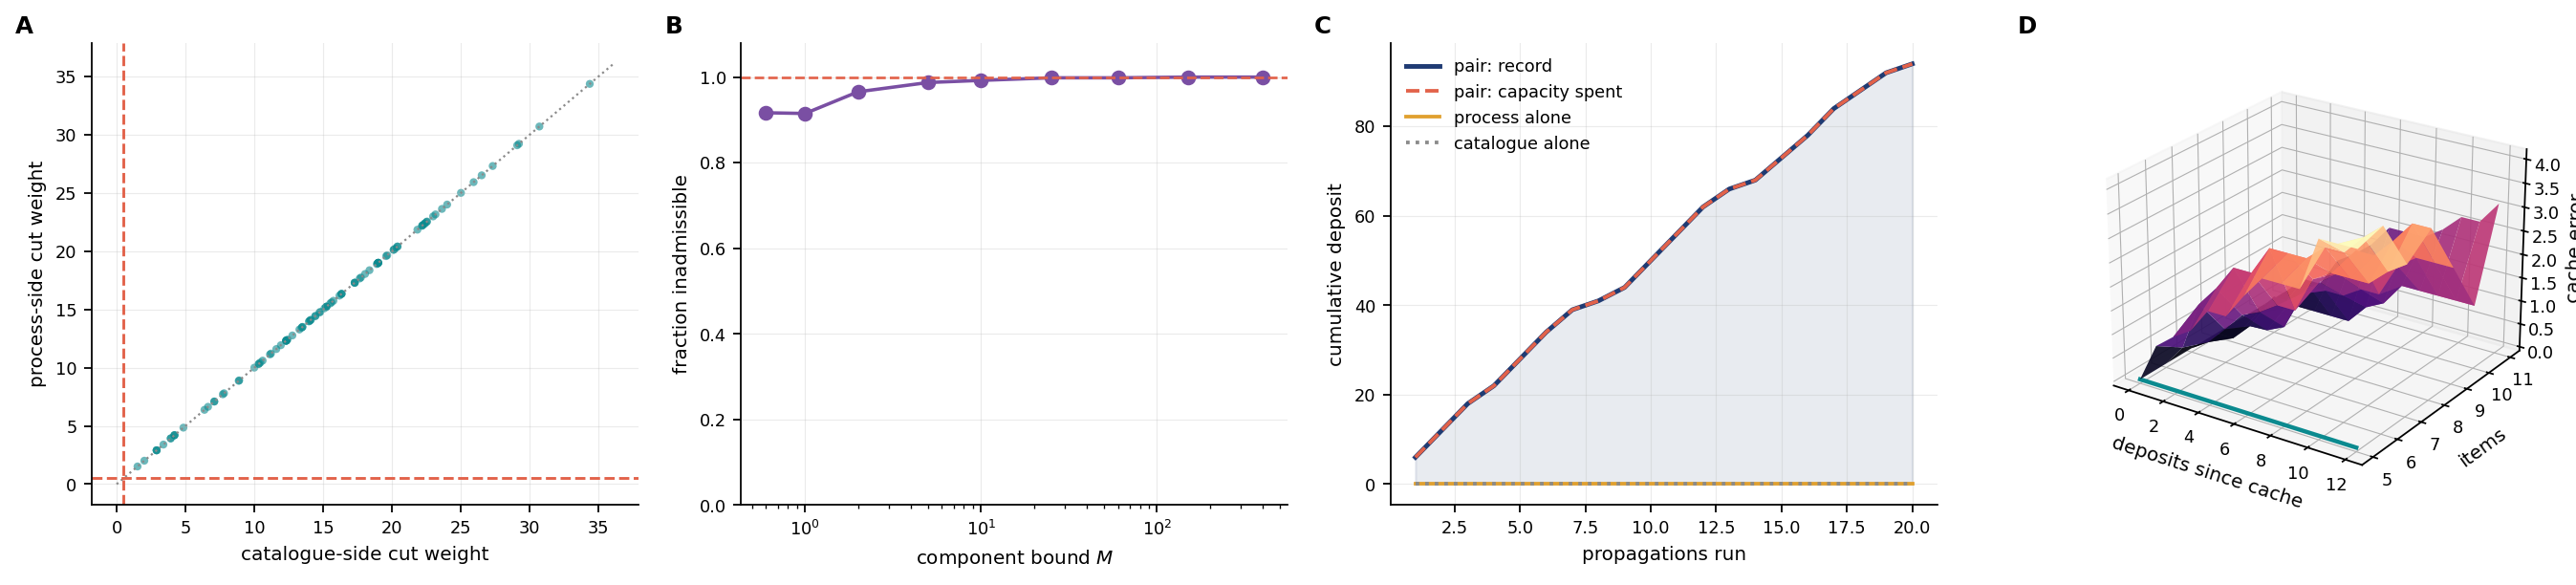
\includegraphics[width=\textwidth]{figures/panel_3_directional.png}
    \caption{\textbf{One Table, Two Directions; and the Deposit That Makes the
    Pair an Individual.}
    (\textbf{A})~Process-side cut weight on the linear $y$-axis versus
    catalogue-side cut weight on the linear $x$-axis, for $200$ outputs drawn
    from $50$ graphs, with the floor marked on both axes (crimson dashed) and
    the identity diagonal in grey. Every output of both regimes is a cut of
    weight $\ge\flo$: $0$ type violations. The two regimes do not merely
    interoperate---they return objects of one type, which is the converse half
    of Theorem~\ref{thm:catalogue-table} (Directional Identity). The forward
    half is verified separately on all $320$ items of the same graphs, with $0$
    mismatches.
    (\textbf{B})~Fraction of admissible representations carrying at least one
    component outside the range a single admissible item could occupy, on the
    linear $y$-axis versus the component bound $M$ on a log $x$-axis ($0.6$ to
    $400$), $3000$ draws per point. The fraction climbs to and remains at $1.0$
    (crimson reference) once $M$ exceeds a few units: inadmissible components
    are the generic case, not an exception, exactly as
    Remark~\ref{rem:virtual-components} asserts. Over $200$ independent trials
    the mean is preserved to a maximum error of $5.0\times10^{-15}$ while
    $98.5\%$ of representations carry an inadmissible component.
    (\textbf{C})~Cumulative deposit on the linear $y$-axis versus propagations
    run on the linear $x$-axis. The pair's record (navy) and consumed capacity
    (crimson dashed) rise together across the run; the process alone (amber)
    and the catalogue alone (grey dotted) remain flat at zero. The shaded band
    between them is what Theorem~\ref{thm:pair-blunts} supplies and neither
    half supplies on its own; the pattern held in all $40$ trials.
    (\textbf{D})~Error of a cached determination as a three-dimensional surface
    (magma) over deposits since caching on the $x$-axis ($0$ to $12$) and item
    count on the $y$-axis ($5$ to $11$), elevation $24^{\circ}$ azimuth
    $-56^{\circ}$. The surface rises away from the teal zero-line, which is the
    pair recomputing against the current graph. Across $40$ trials the cache
    went stale in $21$ and the pair in $0$: the geometry of
    Proposition~\ref{prop:staleness} against
    Corollary~\ref{cor:no-staleness}.}
    \label{fig:panel3}
\end{figure*}

\begin{remark}[Reading the direction]
\label{rem:direction}
The word \emph{directional} names the asymmetry in
\Cref{thm:catalogue-table}. The two regimes are not symmetric alternatives:
the resting regime produces the fixed points of individuation, and the
process regime produces cells the resting regime cannot, precisely because
they depend on a process. The flow of residue is likewise directional---from
propagation into the catalogue, by \Cref{thm:pair-blunts}---and never the
reverse, since by \Cref{thm:monotone} committed structure is not un-committed.
The catalogue accretes; the process side consumes and deposits.
\end{remark}

\subsection{What the pair inherits}

We record, as corollaries, the properties the pair inherits from
Parts~I and~II, since these are what a builder must honour.

\begin{corollary}[No re-presentation]
\label{cor:no-representation}
In a directional pair, a prior propagation is retained as committed edges of
$\Gph$ and is never available as material for a later propagation to reason
about. Hence \Cref{prop:reification} does not apply: there is no operation
that converts a prior propagation into content.
\end{corollary}

\begin{proof}
By \Cref{def:pair} the deposit map commits residue as contacts. By
\Cref{thm:one-use} a committed edge is not re-committed: a second commitment
is either a no-op or a distinct cut event at higher record. There is
therefore no operation returning a prior propagation as an input, and the
hypothesis of \Cref{prop:reification}---that $P$ is re-presented as
content---is unsatisfiable in the pair.
\end{proof}

\begin{corollary}[No staleness]
\label{cor:no-staleness}
Every determination the pair returns is computed against $\Gph$ as it stands
at the record of the determination.
\end{corollary}

\begin{proof}
By \Cref{def:table} a table output is a minimum cut computed in the current
graph, and by \Cref{thm:pair-blunts} every prior propagation has already been
committed into that graph. Hence no output is a determination of an earlier
configuration, and the hypothesis of \Cref{prop:staleness} is unsatisfiable.
\end{proof}

\begin{corollary}[Repeated queries need not agree, and this is correct]
\label{cor:repeat}
Two determinations of the same target at two records need not coincide. The
divergence is not error: by \Cref{thm:pair-blunts} the first determination
committed cuts that altered $\Gph$, so the second is computed against a
different graph.
\end{corollary}

\begin{proof}
Immediate from \Cref{cor:no-staleness} and \Cref{thm:monotone}: the two
determinations are computed at distinct states, and \Cref{def:table} makes
the output a function of the graph.
\end{proof}

\begin{remark}[Reproducibility relocates]
\label{rem:repro}
\Cref{cor:repeat} abandons a familiar expectation deliberately. If repeated
determinations need not agree, what is reproducible? The answer is the
\emph{protocol and its provenance}: which items were present, which process
was run, which contacts were available. Another party reproduces a
determination by reconstituting the same process against the same catalogue
and expects, not the same cut, but a determination of the same protocol whose
differing cuts are themselves data \citep{moreau2013,peng2011,sandve2013}.
This is the sense in which an experimental result is reproducible: not that
the readings coincide, but that the protocol can be re-enacted and the
readings compared \citep{openscience2015}. No theorem depends on the reading.
\end{remark}

% =====================================================================
\part{Construction and Probing}
\label{part:build}
% =====================================================================

% =====================================================================
\section{Construction: the term map is the only declared input}
\label{sec:construction}
% =====================================================================

Everything in Parts~I--III is a theorem about a contact graph. Nothing so far
says where the graph comes from. We now isolate that question, show it is a
single well-defined input, and prove that the calculus is correct for any
value of it---which is what makes a fallible constructor safe to use.

\subsection{The term map}

\begin{definition}[Term map; induced contact graph]
\label{def:term-map}
Let $\mathcal{U}$ be a finite set of \emph{sources}---documents, records,
measurements, prior determinations. A \emph{term map} is a function
$\terms\colon\mathcal{U}\to 2^{\mathcal{D}}$ assigning to each source the
finite set of \emph{distinctions} it draws, valued in a distinction alphabet
$\mathcal{D}$. The \emph{induced contact graph} $\Gph_\terms$ has vertex set
$\mathcal{U}\cup\set{\med}$, a contact $\set{u,v}$ whenever
$\terms(u)\cap\terms(v)\neq\varnothing$ with weight
$\wt(\set{u,v})=f(\abs{\terms(u)\cap\terms(v)})$ for a fixed strictly
increasing $f\colon\N_{>0}\to\R_{\ge\flo}$, and $\med$ adjacent to every
source at weight $\ge\flo$.
\end{definition}

\begin{remark}[What the term map is and is not]
\label{rem:term-map-is}
$\terms$ is a reading of unstructured material. It is not a judgement about
truth, relevance, or importance: it says only which distinctions a source
draws. It is the one place where a component external to the calculus
enters, and \Cref{thm:tau-agnostic} below bounds exactly what damage such a
component can do.
\end{remark}

\begin{theorem}[The calculus is correct for any term map]
\label{thm:tau-agnostic}
Let $\terms$ be any term map and $\Gph_\terms$ its induced contact graph.
Then every result of Parts~I--III holds of $\Gph_\terms$: the floor is
positive, the character invariant is conserved and non-local, the record is
monotone, individuation is symmetric and self-blunting, the table is
well-defined, and the directional identity holds. No result requires
$\terms$ to be accurate, complete, or agreed.
\end{theorem}

\begin{proof}
By \Cref{def:term-map} $\Gph_\terms$ is a finite weighted graph with a
medium vertex adjacent to every item and all weights $\ge\flo$, i.e.\ a
contact graph in the sense of \Cref{def:contact}. \Cref{ax:finite} holds by
finiteness of $\mathcal{U}$ and \Cref{ax:noncompletable} is a premise about
the medium, unaffected by $\terms$. Every theorem of Parts~I--III is derived
from \Cref{def:contact} together with \Cref{ax:finite,ax:noncompletable}
alone, and none inspects the provenance of an edge. Hence all hold.
\end{proof}

\begin{corollary}[Extraction error coarsens; it does not corrupt]
\label{cor:coarsen}
An inaccurate term map yields a contact graph whose cells are coarser or
finer than they would otherwise be, and whose determinations are
correspondingly coarser or finer. It cannot make a determination unsound
relative to the graph it induces, because soundness is a property of the
graph and \Cref{thm:tau-agnostic} holds for every graph.
\end{corollary}

\begin{proof}
Immediate from \Cref{thm:tau-agnostic}: the conclusions are theorems about
$\Gph_\terms$, whatever $\terms$ was.
\end{proof}

\subsection{The floor as a quality readout}

\Cref{cor:coarsen} says an error in $\terms$ is visible as coarseness. We now
show the coarseness is measurable, and measurable \emph{without a reference
graph to compare against}, which is the practical value of the result.

\begin{definition}[Refinement of term maps]
\label{def:refinement}
A term map $\terms'$ \emph{refines} $\terms$, written
$\terms'\preceq\terms$, if for all $u,v$,
$\terms'(u)\cap\terms'(v)\supseteq\terms(u)\cap\terms(v)$: every distinction
$\terms$ draws in common between two sources, $\terms'$ also draws.
\end{definition}

\begin{theorem}[Floor monotonicity]
\label{thm:floor-readout}
If $\terms'\preceq\terms$ then $\flo^{\ast}(\Gph_{\terms'})\ge
\flo^{\ast}(\Gph_{\terms})$: a finer term map induces a system floor at least
as large. Equivalently, the realised system floor is monotone in the
refinement order on term maps.
\end{theorem}

\begin{proof}
Fix an item $v$. By \Cref{def:refinement} every contact present in
$\Gph_\terms$ is present in $\Gph_{\terms'}$ with weight at least as large,
since $f$ is strictly increasing and the shared-distinction count does not
decrease. Any cut separating $v$ from $\med$ in $\Gph_{\terms'}$ therefore has
weight at least that of the corresponding cut in $\Gph_\terms$, so the minimum
over cuts satisfies $\str_{\Gph_{\terms'}}(v)\ge\str_{\Gph_\terms}(v)$.
Taking the minimum over items (\Cref{def:system-floor}) preserves the
inequality.
\end{proof}

\begin{corollary}[Ground-truth-free quality signal]
\label{cor:quality-signal}
The realised system floor $\flo^{\ast}(\Gph_\terms)$ is computable from
$\Gph_\terms$ alone by $\abs{\V}$ minimum-cut computations
\citep{fordfulkerson1956,stoer1997}, and by \Cref{thm:floor-readout} it is
monotone in the quality of $\terms$ under refinement. It therefore serves as
a quality readout for the constructing component that requires no reference
graph and no labelled data.
\end{corollary}

\begin{proof}
Computability is \Cref{def:sepcost} together with the exactness of maximum
flow; monotonicity is \Cref{thm:floor-readout}.
\end{proof}

\begin{remark}[The shape of the guarantee]
\label{rem:quality-honest}
\Cref{cor:quality-signal} is a monotonicity statement, not a calibration.
It says that refining the term map cannot lower the realised floor, so a
system whose floor is not rising under attempted refinement is not being
refined. It does not say that a higher floor is always better---an
over-connected graph in which everything shares distinctions with everything
has a high floor and poor discrimination---so the readout is a signal to be
read alongside cell sizes, not a scalar to be maximised. We state this
explicitly because the temptation to optimise it directly is obvious and
would be an error.
\end{remark}

\subsection{Construction is itself a determination}

Construction is not outside the calculus. It is a determination against the
medium, and the results of \Cref{sec:probing,sec:closure} govern it.

\begin{principle}[Construction discipline]
\label{prin:construction}
A term map should be produced by no fewer than three constructors of distinct
kind, run to closure in the sense of \Cref{def:closure}, with disagreement
between constructors recorded as contested closure
(\Cref{thm:decline}) rather than resolved by adjudication---which by
\Cref{thm:no-verdict} the system cannot perform anyway.
\end{principle}

\begin{remark}[Why three, and why distinct]
\label{rem:three-constructors}
The count and the diversity requirement are not stylistic. \Cref{thm:triangle}
proves that a support structure of fewer than three members is not robust to
the failure of a single member, and \Cref{cor:diversify} proves that repeated
application of one constructor accrues resolution strictly more slowly than
application of distinct ones and may fail to saturate at all. Two
constructors agreeing is mutual definition without external check; five
prompts to one constructor is a single constructor.
\end{remark}

\begin{remark}[Carrying structure, not material]
\label{rem:carry-structure}
Once $\Gph_\terms$ is built, the sources $\mathcal{U}$ need not be carried.
By \Cref{thm:three} the committed contacts retain the \emph{links}---the
information reading---whereas re-supplying the source material would present
the deposits without their links, i.e.\ the entropy reading. Sources are
regenerable from an external substrate given the distinctions that were drawn
from them; committed structure is not regenerable from the sources, because
by \Cref{def:term-map} the same source contributes different contacts in
different graphs. Carry the structure; regenerate the material.
\end{remark}

\begin{figure*}[!htbp]
    \centering
    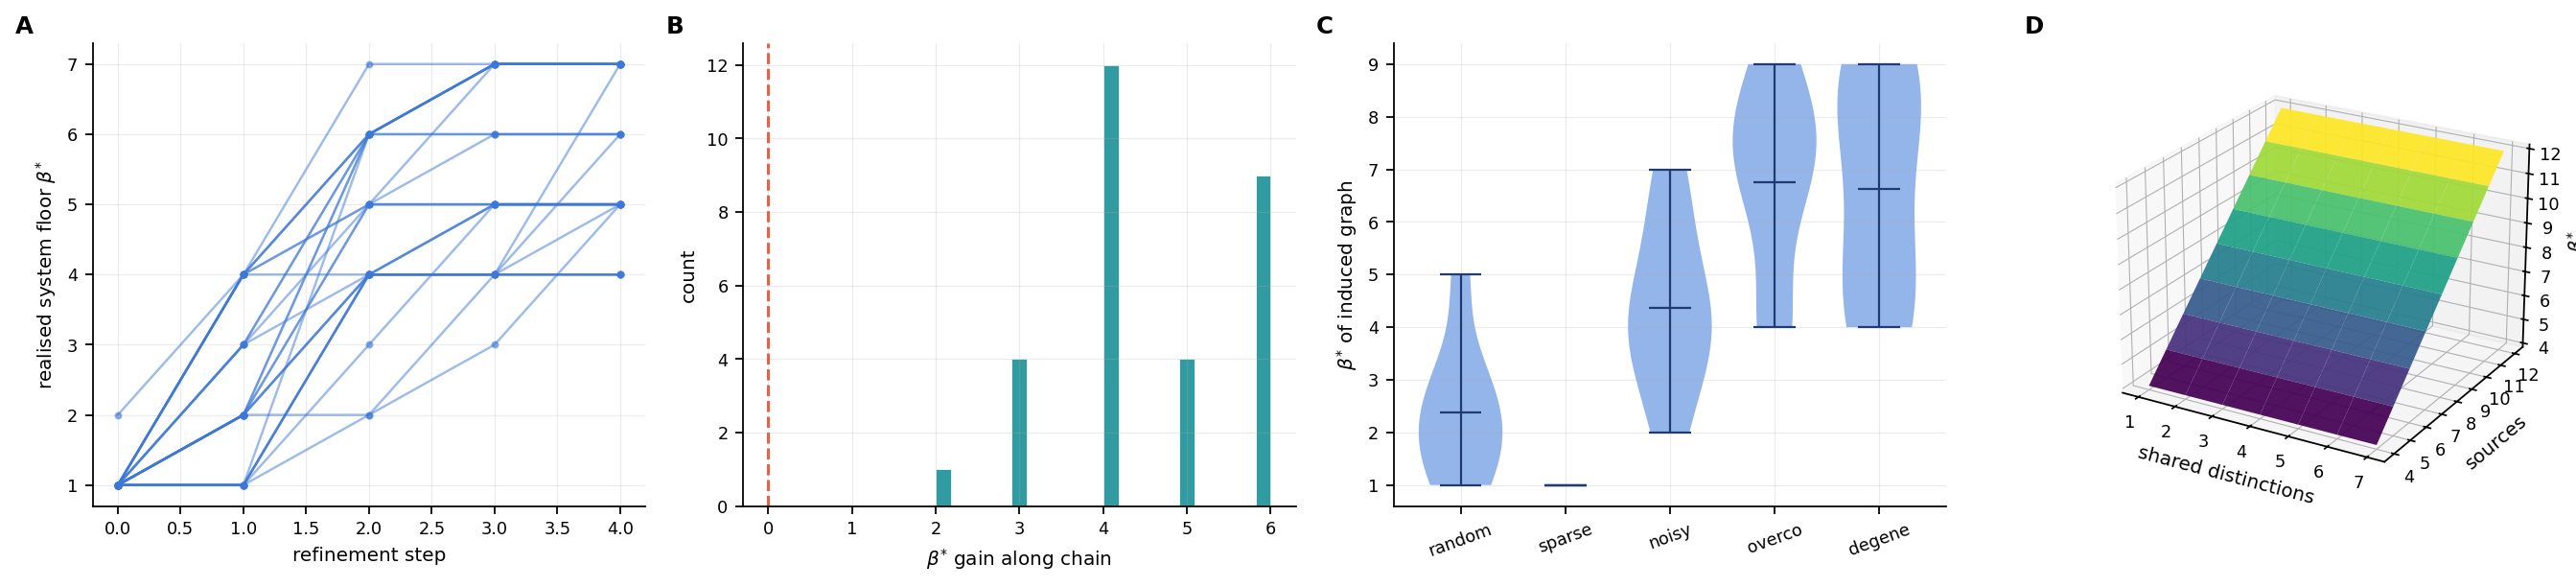
\includegraphics[width=\textwidth]{figures/panel_4_construction.png}
    \caption{\textbf{The Calculus Is Indifferent to the Quality of the Term
    Map, and the Realised Floor Reports That Quality Without a Reference.}
    (\textbf{A})~Realised system floor $\flo^{\ast}$ on the linear $y$-axis
    versus refinement step on the linear $x$-axis ($0$ to $4$), for $26$ of the
    $40$ chains of term maps ordered by the refinement relation of
    Definition~\ref{def:refinement}. Every chain is monotone non-decreasing;
    across all $40$ valid chains there are $0$ monotonicity violations. This is
    the empirical content of Theorem~\ref{thm:floor-readout} (Floor
    Monotonicity).
    (\textbf{B})~Distribution of the floor gain from the coarsest to the finest
    map of each chain, $22$ bins, with the crimson reference at zero. The
    support lies entirely to the right of it: no chain loses floor under
    refinement, and the gains cluster at $4$ to $6$ units.
    (\textbf{C})~Distribution of the realised floor by kind of term map, as
    violins over five deliberately adversarial families---random, sparse,
    noisy, over-connected, and degenerate (every source drawing identical
    distinctions), $60$ maps in total. Every family induces a graph on which
    the floor, the edge bound, relabelling invariance, and cut non-emptiness
    all hold: $0$ failures, the content of Theorem~\ref{thm:tau-agnostic}. The
    families differ markedly in the floor they induce, which is the coarsening
    of Corollary~\ref{cor:coarsen} made visible. Note that the degenerate
    family induces among the \emph{highest} floors while discriminating worst:
    the floor is a monotone signal of refinement, not a quantity to maximise
    (Remark~\ref{rem:quality-honest}).
    (\textbf{D})~Realised floor as a three-dimensional surface (viridis) over
    the number of shared distinctions on the $x$-axis ($1$ to $7$) and the
    number of sources on the $y$-axis ($4$ to $12$), each cell the mean of five
    induced graphs, elevation $23^{\circ}$ azimuth $-60^{\circ}$. The surface
    is smooth and monotone in the shared-distinction axis: more shared
    structure yields a higher floor and correspondingly coarser cells, across
    the whole two-dimensional parameter region.}
    \label{fig:panel4}
\end{figure*}

% =====================================================================
\section{Probing: many determiners over one graph}
\label{sec:probing}
% =====================================================================

A determination need not be made by a single mechanism. We develop the
algebra of multiple determiners---\emph{probes}---acting on one contact
graph, and prove four things about them: how they compose, how many are
required, how a finite budget should be divided among them, and why finding
and pruning cannot be one operation.

\subsection{Probes and probing power}

\begin{definition}[Probe]
\label{def:probe}
A \emph{probe} toward a target $x^{\star}$ is a partial map
$\gamma\colon\V\rightharpoonup\V$ on items such that, where defined,
applying $\gamma$ to an item $x$ commits a contact and yields $\gamma(x)$;
that is, a probe realises a contact operation (\Cref{def:contact-op}).
\end{definition}

\begin{definition}[Probing power]
\label{def:power}
The \emph{probing power} of $\gamma$ toward $x^{\star}$ at an item $x$ is the
fraction of above-floor alignment it closes:
\[
\pot(\gamma,x,x^{\star})\;=\;
\frac{\al(x,x^{\star})-\al(\gamma(x),x^{\star})}
     {\al(x,x^{\star})-\flo/\Om}\;\in\;[0,1].
\]
A probe is \emph{inert} if $\pot=0$ and \emph{absolute} if $\pot=1$.
\end{definition}

\begin{lemma}[Power is bounded]
\label{lem:power-bound}
$\pot\in[0,1]$ for every probe, item, and target.
\end{lemma}

\begin{proof}
By \Cref{lem:align-floor}, $\al(\gamma(x),x^{\star})\ge\flo/\Om$, so the
numerator never exceeds the denominator. Non-negativity holds for probes
directed toward $x^{\star}$; a probe that increases alignment is assigned
$\pot=0$ by convention, not being a probe toward $x^{\star}$ in the operative
sense.
\end{proof}

\begin{remark}[Probes are structurally unconstrained]
\label{rem:probe-neutral}
\Cref{def:probe,def:power} inspect nothing about a probe beyond its action on
items and the alignment it closes. A probe may be a local computation, a
remote retrieval, a deterministic rule, or an inference by a trained model:
none of the results below distinguishes these cases, because none of the
definitions refers to anything but $\gamma$'s action. A classification of
probes by kind is useful for scheduling---expected cost and latency
differ---but carries no weight in the theory.
\end{remark}

\subsection{Composition is multiplicative}

\begin{theorem}[Multiplicative composition]
\label{thm:multiplicative}
For probes $\gamma_1,\dots,\gamma_n$ applied in sequence, each to the output
of the last, with powers $\pot_1,\dots,\pot_n$ toward a fixed target, the
composite power is
\[
\pot(\gamma_1\diamond\cdots\diamond\gamma_n)\;=\;1-\prod_{i=1}^{n}(1-\pot_i).
\]
\end{theorem}

\begin{proof}
Let $r_0=\al(x_0,x^{\star})-\flo/\Om$ be the initial above-floor gap.
Applying $\gamma_1$ leaves gap $r_1=(1-\pot_1)r_0$ by \Cref{def:power};
applying $\gamma_2$ leaves $r_2=(1-\pot_2)(1-\pot_1)r_0$; by induction
$r_n=\prod_i(1-\pot_i)r_0$. The fraction of the initial gap closed is
$1-r_n/r_0$, which is the composite power by \Cref{def:power} applied to the
chain as a single probe.
\end{proof}

\begin{corollary}[Diminishing returns of repetition]
\label{cor:diminishing}
Repeating one probe of power $\pot$ a total of $n$ times gives composite power
$1-(1-\pot)^n$: strictly increasing, convergent to $1$, never reaching it for
finite $n$. Each repetition closes a strictly smaller absolute fraction of the
remaining gap than the last.
\end{corollary}

\begin{corollary}[Saturation dichotomy]
\label{cor:saturation}
A chain of probes with powers $(\pot_i)_{i\ge1}$ drives the residual gap to
zero in the limit if and only if $\sum_i\pot_i=\infty$.
\end{corollary}

\begin{proof}
The residual fraction after $n$ probes is $\prod_{i\le n}(1-\pot_i)$. Taking
logarithms, $\sum_{i\le n}\log(1-\pot_i)\to-\infty$ if and only if
$\sum_i\pot_i=\infty$, since $-\log(1-\pot)\asymp\pot$ for small $\pot$ and
the comparison test applies; this is a dichotomy of Borel--Cantelli type
\citep{borel1909,cantelli1917}.
\end{proof}

\begin{corollary}[Diversify, do not repeat]
\label{cor:diversify}
A chain of $n$ distinct probes with powers $\pot_1,\dots,\pot_n$ attains
composite power $1-\prod_i(1-\pot_i)$, which strictly exceeds the composite
power $1-(1-\pot_j)^n$ of $n$ repetitions of any single member $\gamma_j$
whenever some $\pot_i>\pot_j$. A chain of near-duplicate probes accrues power
slowly and, if its powers decay fast enough, fails to saturate even in
principle (\Cref{cor:saturation}).
\end{corollary}

\begin{proof}
Both composite powers are given by \Cref{thm:multiplicative}; the comparison
is the elementary fact that $\prod_i(1-\pot_i)<(1-\pot_j)^n$ when some factor
is strictly smaller than $(1-\pot_j)$. Failure to saturate is
\Cref{cor:saturation} applied to a summable power sequence.
\end{proof}

\subsection{Coherence requires three}

Multiplicativity presumes probes directed at one target. We now show that
robustness against the failure of a single probe requires a support structure
of at least three members.

\begin{definition}[Support; support graph]
\label{def:support}
For probes $\gamma_i,\gamma_j$ toward a common target, say $\gamma_j$
\emph{supports} $\gamma_i$ at threshold $\theta\in(0,1]$ if the presence of
$\gamma_j$'s result does not reduce, and to degree $\ge\theta$ reinforces, the
alignment shift toward the target induced by $\gamma_i$. The \emph{support
graph} $G$ has an edge $j\to i$ whenever $\gamma_j$ supports $\gamma_i$ at
$\theta$.
\end{definition}

\begin{theorem}[Linear support fails]
\label{thm:linear-fails}
No finite chain $\gamma_1\to\gamma_2\to\cdots\to\gamma_n$ in which each
probe's contribution is justified only by the next, and the terminal probe by
nothing internal to the chain, is robust to removal of the terminal probe.
\end{theorem}

\begin{proof}
The terminal probe $\gamma_n$ has no incoming support edge in $G$; its
contribution rests on nothing internal to the chain. Removing $\gamma_n$
leaves $\gamma_{n-1}$ unsupported, and by induction each successive removal
leaves the next probe unsupported. The chain's claim to be grounded is
contingent on retaining every member, and a single removal at the terminus
collapses the justification with no internal check to prevent it.
\end{proof}

\begin{theorem}[Coherence requires three mutually supporting probes]
\label{thm:triangle}
\leavevmode
\begin{enumerate}[label=\textup{(\roman*)},leftmargin=2.0em,itemsep=2pt]
\item \emph{Necessity.} If a set of probes brings a determination's terminal
alignment within any margin of the floor and remains so after the failure of
any single probe, its support graph contains a directed cycle of length
$\ge3$.
\item \emph{Sufficiency.} Three probes mutually supporting one another at
threshold $\theta>\tfrac12$, forming a strongly connected triangle in $G$,
ground the determination robustly: their combined shift toward the target
survives the removal of any single member.
\end{enumerate}
\end{theorem}

\begin{proof}
(i) By \Cref{thm:linear-fails} no acyclic support structure is robust to
removal of its terminal member; an acyclic $G$ has a source probe with no
incoming support, and the same argument applies to it. A $1$-cycle is
self-support and vacuous. A $2$-cycle is mutual definition between exactly two
probes with no independent third check, and fails the majority condition
$\theta>\tfrac12$: removing either leaves one probe, itself unsupported.
Hence the shortest support cycle compatible with robustness has length $\ge3$.

(ii) In a strongly connected triangle each probe is supported by the other
two; with $\theta>\tfrac12$ the two supporters jointly exceed any single
dissenting signal. Removing one leaves the remaining two still mutually
supporting each other directly, above a reduced but positive effective
threshold, so the shift toward the target persists.
\end{proof}

\begin{corollary}[Coherence is ordinally decidable]
\label{cor:ordinal}
Whether a set of probes is coherent in the sense of \Cref{thm:triangle} is
decidable from the \emph{signs} of pairwise support relations alone---whether
each pair reinforces or undercuts the other's shift---with no access to
probing-power magnitudes.
\end{corollary}

\begin{proof}
\Cref{thm:triangle} is stated and proved entirely in terms of the
directed-graph structure of $G$ (cycle existence and length) and the threshold
comparison $\theta>\tfrac12$, both determined by the signed support relation
of \Cref{def:support} and not by any numerical power.
\end{proof}

\subsection{Dividing a finite probing budget}

Probes cost. We now solve the allocation problem, first in the discrete
regime and then in the continuous one, and note precisely when each applies.

\begin{definition}[Probe selection instance]
\label{def:selection}
Given probes $\gamma_1,\dots,\gamma_k$ with floors $\flo_i$ (the residual each
leaves) and per-invocation costs $c_i>0$, and a budget $B>0$, the
\emph{selection problem} is to choose $S\subseteq\set{1,\dots,k}$ minimising
the composite residual $\Om\prod_{i\in S}(1-\flo_i/\Om)$ subject to
$\sum_{i\in S}c_i\le B$.
\end{definition}

\begin{theorem}[Selection is a $0/1$ knapsack]
\label{thm:knapsack}
The selection problem is equivalent to a $0/1$ knapsack with values
$v_i=-\log(1-\flo_i/\Om)>0$, costs $c_i$, and capacity $B$. It is solvable
exactly by dynamic programming in $\mathcal{O}(kB)$ time and space, and the
value-density greedy rule---admit probes in decreasing order of $v_i/c_i$---is
optimal under the linear relaxation and within a factor
$(1-c_{\max}/B)$ of optimal for the integral problem
\citep{dantzig1957,kellerer2004,sahni1975}.
\end{theorem}

\begin{proof}
Taking logarithms of the objective,
$\log\bigl(\Om\prod_{i\in S}(1-\flo_i/\Om)\bigr)=\log\Om-\sum_{i\in S}v_i$,
so minimising the composite residual is maximising $\sum_{i\in S}v_i$ subject
to the budget, which is the stated knapsack verbatim. The dynamic program is
standard \citep{cormen2009}; the greedy bound and the fully polynomial
approximation scheme are \citet{dantzig1957} and \citet{sahni1975}.
\end{proof}

\begin{corollary}[Selection priority]
\label{cor:priority}
A probe with residual $\flo_i$ and cost $c_i$ has selection priority
\[
\varrho_i\;=\;\frac{1}{c_i}\log\frac{\Om}{\Om-\flo_i},
\]
and probes are admitted in decreasing order of $\varrho_i$.
\end{corollary}

\begin{definition}[Probing allocation; gain profile]
\label{def:alloc}
Suppose instead that a probe may be applied to a graded extent: an
\emph{allocation} is a vector $\alloc=(a_1,\dots,a_k)\in[0,\infty)^k$ with
$\sum_i a_i\le\att$ for a budget $\att>0$, where $a_i$ is the effort spent on
probe $i$. The \emph{gain profile} $\gain_i\colon[0,\infty)\to[0,\infty)$
gives the above-floor alignment $\gain_i(a_i)$ that probe $i$ removes at
effort $a_i$, with $\gain_i(0)=0$. The value of an allocation is
$G(\alloc)=\sum_i\gain_i(a_i)$.
\end{definition}

\begin{axiom}[Diminishing returns within a probe]
\label{ax:concave}
Each gain profile $\gain_i$ is concave and nondecreasing.
\end{axiom}

\begin{remark}[This premise is about the environment, not the system]
\label{rem:concave-honest}
\Cref{ax:concave} is the one premise in this paper that is a claim about the
problem being probed rather than about the structure doing the probing. It
says that the second unit of effort spent on a probe removes no more alignment
than the first. Where it fails---where a probe has a threshold below which it
returns nothing and above which it returns a great deal---\Cref{thm:waterfill}
does not apply and the discrete selection of \Cref{thm:knapsack} is the
correct model. We flag the dependence explicitly; every other result in the
paper is independent of it.
\end{remark}

\begin{theorem}[Optimal division is water-filling]
\label{thm:waterfill}
Under \Cref{ax:concave}, the value-maximising allocation solves
$\max_{\alloc\ge0,\ \sum_i a_i\le\att}\sum_i\gain_i(a_i)$, and there is a
single \emph{shadow price} $\price\ge0$ such that the optimum satisfies
\[
\gain_i'(a_i^{\star})=\price\ \text{ if } a_i^{\star}>0,
\qquad
\gain_i'(0)\le\price\ \text{ if } a_i^{\star}=0 .
\]
The system equalises marginal gain across all engaged probes at the price
$\price$, and drops any probe whose first unit of effort returns less than
$\price$. The price is nonincreasing in the budget $\att$ and nondecreasing in
the number and richness of competing probes; if the budget is not exhausted at
the optimum then $\price=0$.
\end{theorem}

\begin{proof}
The objective is concave as a sum of concave functions and the feasible set
$\set{\alloc\ge0:\sum_i a_i\le\att}$ is compact and convex, so a maximiser
exists \citep{boyd2004}. Form the Lagrangian
$L=\sum_i\gain_i(a_i)-\price(\sum_i a_i-\att)+\sum_i\mu_i a_i$ with
$\price\ge0$, $\mu_i\ge0$. Stationarity gives
$\gain_i'(a_i)-\price+\mu_i=0$ with complementary slackness $\mu_i a_i=0$ and
$\price(\sum_i a_i-\att)=0$ \citep{kuhntucker1951}. For $a_i^{\star}>0$,
$\mu_i=0$ yields $\gain_i'(a_i^{\star})=\price$; for $a_i^{\star}=0$,
$\mu_i\ge0$ yields $\gain_i'(0)\le\price$. Sufficiency of the conditions for
a global optimum follows from concavity. Budget monotonicity: relaxing $\att$
enlarges the feasible set, so the optimal value is nondecreasing and, being
concave in $\att$, its marginal $\price$ is nonincreasing. Adding a probe or
raising a profile tightens the binding budget and raises the level at which
margins equalise. If the budget is slack at the optimum, its multiplier is
zero.
\end{proof}

\begin{corollary}[Every probe engaged, at a price]
\label{cor:engaged}
At the optimum the system spends positive effort in exactly the probes whose
marginal gain at zero exceeds $\price$, and none in the rest; within engaged
probes it holds every marginal gain equal to $\price$. Thus all engaged
probes are working simultaneously, at graded effort, and $\price$ is a single
readable scalar for how loaded the system is. A probe whose entry margin only
marginally exceeds $\price$ receives a floor-sized allocation---the boundary
case of minimal engagement.
\end{corollary}

\begin{figure*}[!htbp]
    \centering
    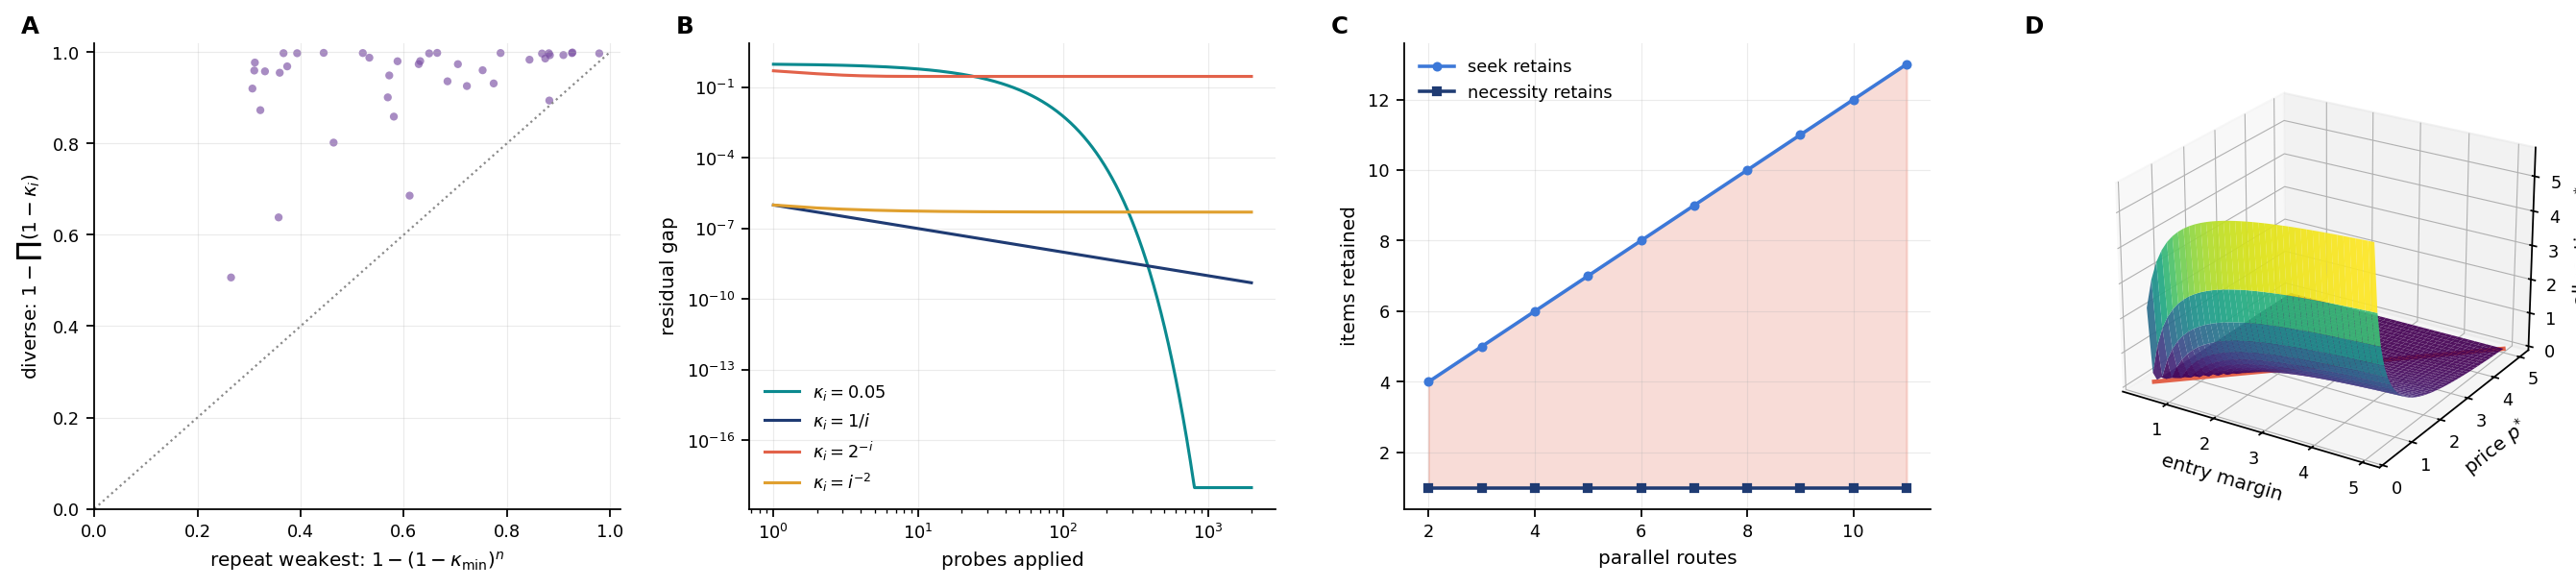
\includegraphics[width=\textwidth]{figures/panel_5_probing.png}
    \caption{\textbf{Probes Compound Rather Than Vote, Saturate Only Under a
    Divergent Sum, and Divide a Budget at a Single Price.}
    (\textbf{A})~Composite power of a chain of distinct probes,
    $1-\prod_i(1-\pot_i)$, on the linear $y$-axis versus the composite power of
    repeating its weakest member the same number of times,
    $1-(1-\pot_{\min})^{n}$, on the linear $x$-axis, over $300$ instances with
    the identity diagonal in grey. Every point lies strictly above the
    diagonal---$300$ of $300$, with no ties---so diversification strictly
    dominates repetition (Corollary~\ref{cor:diversify}). The underlying
    composition law is verified separately on $400$ chains to a maximum
    absolute error of $1.1\times10^{-16}$ (Theorem~\ref{thm:multiplicative}).
    (\textbf{B})~Residual gap on a log $y$-axis versus probes applied on a log
    $x$-axis ($1$ to $2000$), for four canonical power sequences. The two with
    divergent sums---constant $\pot_i=0.05$ (teal) and harmonic $\pot_i=1/i$
    (navy)---drive the residual toward zero; the two with convergent
    sums---geometric $\pot_i=2^{-i}$ (crimson) and inverse-square
    $\pot_i=i^{-2}$ (amber)---plateau strictly above it and stay there. At a
    horizon of $4000$ probes all four sequences match the prediction of
    Corollary~\ref{cor:saturation}: $0$ mismatches.
    (\textbf{C})~Items retained on the linear $y$-axis versus parallel routes
    on the linear $x$-axis ($2$ to $11$), on the diamond witness of
    Theorem~\ref{thm:separation-operators}. The $\seek$ operator (steel) climbs
    linearly from $4$ to $13$ while $\nec$ (navy) stays flat at $1$; the shaded
    region between them is the over-retention a reachability-only mechanism
    incurs, growing from $3$ to $12$ items. On the chain witness the
    complementary identity holds at every tested length: every interior item is
    necessary and the terminal leaf is reachable yet redundant. Over $60$
    random graphs the containment $\nec\subseteq\reach$ holds without
    exception, with a strictly positive gap in $57$, and necessity coincides
    with domination on all $211$ non-seed items checked
    (Corollary~\ref{cor:no-single}).
    (\textbf{D})~Optimal allocation $a_i^{\star}$ as a three-dimensional
    surface (viridis) over entry margin $\gain_i'(0)$ on the $x$-axis ($0.4$ to
    $5.0$) and shadow price $\price$ on the $y$-axis ($0.25$ to $5.0$),
    elevation $24^{\circ}$ azimuth $-58^{\circ}$. The surface rises with margin
    and falls with price, collapsing to the zero floor along the crimson line
    where the entry margin meets the price---the sharp dropout boundary of
    Theorem~\ref{thm:waterfill}. Across $120$ convex instances the stationarity
    conditions hold, the budget is respected, the dropout boundary is sharp,
    and the price is nonincreasing in the budget and nondecreasing in the probe
    count, in $120$ of $120$ cases each.}
    \label{fig:panel5}
\end{figure*}

\begin{proof}
Immediate from the stationarity conditions of \Cref{thm:waterfill}: the
support of $\alloc^{\star}$ is $\set{i:\gain_i'(0)>\price}$, margins on the
support equal $\price$, and $\price$ falls as $\att$ rises.
\end{proof}

\begin{remark}[Selection versus allocation]
\label{rem:selection-vs-alloc}
\Cref{thm:knapsack} and \Cref{thm:waterfill} are the discrete and continuous
faces of one problem. Where a probe is an all-or-nothing invocation, selection
is a knapsack and probes take turns. Where a probe admits graded effort and
\Cref{ax:concave} holds, allocation is water-filling and every probe above the
price works at once. The knapsack is the relaxation's boundary: a probe
dropped at $a_i^{\star}=0$ is a probe excluded from the knapsack's chosen set.
\end{remark}

\subsection{Finding and pruning are different operations}

The last structural result about probing concerns architecture. We show that
locating what bears on a target and determining what may be discarded are
distinct computations, so no single mechanism performs both.

\begin{definition}[Reachability]
\label{def:reach}
Seed a frontier with the target's distinctions. An item is \emph{reachable at
distance $0$} if it shares a distinction with the target, and at distance
$d+1$ if it is not reachable at distance $\le d$ and shares a distinction with
some item reachable at distance $\le d$. Write $\reach(x^{\star})$ for the set
of reachable items.
\end{definition}

\begin{definition}[Resolution functional; contribution; necessity]
\label{def:contribution}
Let $\Res(x^{\star}\mid W)$ be a \emph{resolution functional} on retained sets
$W$: a monotone measure of how much of the target's neighbourhood the retained
items recover, increasing as items are added. The canonical choice is
$\Res(x^{\star}\mid W)=\abs{\reach_W(x^{\star})}$. The \emph{contribution} of
$u\in W$ is
\[
\varsigma(u,x^{\star})\;=\;\Res(x^{\star}\mid W)-\Res\bigl(x^{\star}\mid W\setminus\set u\bigr)\;\ge\;0,
\]
and $u$ is \emph{necessary} if $\varsigma>0$, \emph{purposeless} if
$\varsigma=0$.
\end{definition}

\begin{remark}[The orientation of the functional matters]
\label{rem:orientation}
$\Res$ must \emph{grow} with resolving power, so that removing a load-bearing
item lowers it and contributions are non-negative. A minimum cut of the target
against the medium has the wrong orientation for this role: deleting an item
deletes edges, which can only shrink a cut, making every contribution
non-positive. The reachable-slice measure, or any monotone measure of
recovered neighbourhood, has the correct sign.
\end{remark}

\begin{proposition}[Necessity is contained in reachability]
\label{prop:nec-subset}
$\nec(x^{\star})\subseteq\reach(x^{\star})$: an item the target cannot reach
is never necessary. The reverse inclusion fails in general.
\end{proposition}

\begin{proof}
If $u\notin\reach(x^{\star})$ then no path of shared distinctions connects $u$
to the target, so removing $u$ deletes only edges incident to $u$, none of
which lies on any path from the target into its reachable neighbourhood.
Hence $\Res(x^{\star}\mid W\setminus\set u)=\Res(x^{\star}\mid W)$ and
$\varsigma=0$. For failure of the reverse inclusion, see
\Cref{thm:separation-operators}(iii).
\end{proof}

\begin{proposition}[Necessity is domination]
\label{prop:domination}
A non-seed item is necessary for a target exactly when it \emph{dominates}
some reachable item---lies on every path from the target to it. Domination is
computable in near-linear time \citep{lengauer1979}.
\end{proposition}

\begin{proof}
If $u$ dominates $r$, every path from the target to $r$ passes through $u$, so
removing $u$ removes $r$ from the reachable set and strictly lowers
$\Res$. Conversely if $u$ dominates nothing, then for every reachable $r$
there is a path from the target to $r$ avoiding $u$, so removing $u$ leaves
the reachable set unchanged and $\varsigma=0$.
\end{proof}

\begin{remark}[Two things the measurement must get right]
\label{rem:contribution-care}
\Cref{def:contribution} compares the resolution of the retained set against
that of the set with $u$ removed, and the comparison must be taken over the
items \emph{other than} $u$. Counting $u$'s own disappearance from the
reachable set gives every reachable item a contribution of at least one and
collapses $\nec$ onto $\seek$---which is exactly the degeneracy
\Cref{thm:separation-operators} forbids, and which the validation suite
detected as a failure before the measurement was corrected
(\Cref{rem:validation-boundaries}).

The seed is a genuine boundary case rather than an artefact. A seed is the
target's only point of entry and is load-bearing by definition; where a seed
reaches nothing but itself it dominates no item while remaining necessary.
\Cref{prop:domination} is therefore stated for non-seed items, and a system
computing necessity must treat seeds separately rather than by the domination
test.
\end{remark}

\begin{theorem}[Separation of finding and pruning]
\label{thm:separation-operators}
The operators $\seek(x^{\star})=\reach(x^{\star})$ and
$\nec(W,x^{\star})=\set{u\in W:\varsigma(u,x^{\star})>0}$ compute distinct
quantities and are not reducible to one another by a single pass:
\begin{enumerate}[label=\textup{(\roman*)},leftmargin=2.0em,itemsep=1pt]
\item $\seek$ is a forward reachability from the target---a growth from a
seed---computing what the target \emph{touches};
\item $\nec$ is a backward ablation---a removal test against a retained
set---computing what a drop \emph{changes};
\item the two disagree: there exist items that $\seek$ marks reachable and
$\nec$ marks purposeless, and the discrepancy is recoverable from neither
operator's output alone.
\end{enumerate}
\end{theorem}

\begin{proof}
(i) and (ii) are the definitions, and their computational shapes are
opposite: a seed-and-grow traversal versus a per-item ablation. (iii)
Construct a redundant reachable item. Let a target distinction be shared by
two items $u_1,u_2$, each also joined to a common item $r$, so both lie on a
path from the target to $r$. Both are in $\seek(x^{\star})$. But if $r$ is
reachable via $u_1$ alone, removing $u_2$ leaves $\Res$ unchanged, so $u_2$ is
reachable yet purposeless: $u_2\in\seek$ and $u_2\notin\nec$. The output of
$\seek$---the reachable set---does not record which of its members are
redundant, and the output of $\nec$---the necessary set---does not record the
reachable-but-redundant items it excluded. Neither output determines the
other.
\end{proof}

\begin{corollary}[No single-mechanism probing]
\label{cor:no-single}
A mechanism running only $\seek$ over-retains: it keeps reachable-but-%
redundant items, wasting budget. A mechanism running only $\nec$ has nothing
to ablate against, since $\varsigma$ is defined relative to a retained set.
Correct probing requires both, in the order $\nec\circ\seek$.
\end{corollary}

\begin{proof}
Over-retention is \Cref{thm:separation-operators}(iii). The dependence of
$\nec$ on a retained set is \Cref{def:contribution}, whose natural argument is
$\seek(x^{\star})$.
\end{proof}

\begin{remark}[Consequence for retrieval architectures]
\label{rem:retrieval}
Retrieval-augmented generation \citep{lewis2020} implements $\seek$ alone:
it fetches a relevant subset per query. \Cref{cor:no-single} identifies what
is structurally missing---an operator answering \emph{what may be
discarded}---and \Cref{thm:separation-operators} shows it cannot be obtained
by making the retriever better, because it is a different computation. No
theorem depends on the comparison.
\end{remark}

% =====================================================================
\section{Termination: closure, and the honest decline}
\label{sec:closure}
% =====================================================================

\Cref{thm:no-verdict} showed the system cannot issue a verdict. We now supply
what it \emph{can} report, and prove the stopping rule is not a confidence
threshold.

\begin{definition}[Reachable class set]
\label{def:class-set}
Fix a seed $v_0$ and a process graph whose available probes may be extended
over time. At a given stage, let $\Cell(v_0)$ denote the set of targets
reachable by some admissible propagation of $v_0$ through the probes invoked
so far, partitioned into equivalence classes under
endpoint-indistinguishability (\Cref{cor:gauge}).
\end{definition}

\begin{definition}[Closure]
\label{def:closure}
A determination from seed $v_0$ is \emph{closed} at a given stage if, for
every probe available but not yet invoked, extending by that probe cannot add
a new equivalence class to $\Cell(v_0)$: every further admissible propagation
reachable via it terminates in a class already present.
\end{definition}

\begin{theorem}[Closure is strictly stronger than a confidence threshold]
\label{thm:closure-stronger}
There exist process graphs and thresholds $\theta$ such that a propagation's
terminal alignment satisfies a fixed confidence criterion while the
determination is not closed in the sense of \Cref{def:closure}: a
not-yet-invoked probe is available whose propagation reaches a target in a
distinct equivalence class.
\end{theorem}

\begin{proof}
Construct a process graph with two disjoint item clusters $A$ and $B$, each
internally dense---many low-cost internal contacts---and each connected to
the medium by a single probe, $\gamma_A$ and $\gamma_B$, of equal weight. A
propagation via $\gamma_A$ alone terminates at a representative
$x^{\star}_A\in A$ with terminal alignment
$\al(x^{\star}_A,x^{\star}_A)=\flo/\Om$, satisfying any fixed threshold
$\theta\le1$ trivially, since by \Cref{thm:admissibility} a propagation's
terminal alignment to its own target is always at the floor. Yet $\gamma_B$,
not yet invoked, reaches $x^{\star}_B\in B$, in a distinct equivalence class
from $x^{\star}_A$: the two clusters have independent internal structure, so
their resting cuts against the medium differ and they are not
endpoint-indistinguishable. Hence the confidence criterion is satisfied after
$\gamma_A$ alone while the determination is not closed.
\end{proof}

\begin{remark}[The failure mode the theorem isolates]
\label{rem:closure-failure}
\Cref{thm:closure-stronger} formalises a familiar defect of
threshold-stopping. A single early source may report high confidence purely
because it is internally self-consistent---as any single cluster is, having
only committed contacts within itself and one to the medium---while a second,
independent source would reach an entirely different conclusion. Closure
requires that \emph{every} available further probe be checked to land in an
already-reached class before stopping. It is not that the current
determination looks confident, but that the space of determinations has
stopped producing new destinations.
\end{remark}

\begin{theorem}[Convergent closure or contested closure]
\label{thm:decline}
Every determination over a finite probe registry terminates in exactly one of
two states:
\begin{enumerate}[label=\textup{(\roman*)},leftmargin=2.0em,itemsep=2pt]
\item \textbf{Convergent closure}: $\Cell(v_0)$ stabilises to a single
equivalence class, and the determination reports that class's representative;
\item \textbf{Contested closure}: $\Cell(v_0)$ stabilises---no further probe
adds a class---but contains more than one class, and the determination
reports \emph{decline}: no single sufficient determination exists, together
with the distinct classes found.
\end{enumerate}
No determination over a finite registry runs forever without reaching one of
these two states.
\end{theorem}

\begin{proof}
The probe registry available at any call is finite, so the set of
propagations reachable from $v_0$ is finite, and hence $\Cell(v_0)$---a
partition of a finite set of reachable targets---is finite and can grow by
only finitely many steps before every remaining probe has been tried against
every currently-reached class. At that point \Cref{def:closure} is satisfied
by exhaustion, so closure is reached in finitely many steps. If the
stabilised $\Cell(v_0)$ has exactly one class, the determination is
convergently closed; if more than one, then by \Cref{cor:gauge} each class is
internally endpoint-indistinguishable while the classes disagree with one
another, so no single sufficient determination is licensed and decline is
reported. The two cases are exhaustive and mutually exclusive on a partition
with at least one class, and at least one class exists once any propagation is
admissible.
\end{proof}

\begin{corollary}[Decline is a first-class output]
\label{cor:decline-first-class}
Contested closure is a correctly-terminating outcome carrying the distinct
classes found. It is not a failure to be retried, and by \Cref{thm:no-verdict}
the system could not adjudicate between the classes even if instructed to.
\end{corollary}

\begin{proof}
\Cref{thm:decline}(ii) establishes contested closure as one of two terminal
states of a terminating procedure, and \Cref{thm:no-verdict} forbids the
system from selecting among the classes.
\end{proof}

\begin{remark}[What contested closure is worth]
\label{rem:contested-value}
A determination that ends in contested closure has located precisely where
independent probing diverges. That is ordinarily more valuable than either
class alone, and is exactly the information a threshold-stopping procedure
discards: by \Cref{thm:closure-stronger} such a procedure would have halted
at whichever class it reached first and reported it as sufficient. No theorem
depends on the reading.
\end{remark}

\begin{corollary}[Anytime discipline]
\label{cor:anytime}
The correct stopping condition is non-resolution against the floor, not
budget exhaustion: a determination whose reachable propagations do not settle
the target's distinctions to within $\flo$ should descend further or decline,
never fabricate. This sharpens the anytime stance
\citep{dean1988,zilberstein1996} by moving the stopping criterion from
elapsed effort to structural closure.
\end{corollary}

\begin{proof}
By \Cref{cor:no-sharp} ``resolved'' is a region with a positive boundary; a
target whose reachable propagations never enter that region is genuinely
unresolved by the current structure, and \Cref{thm:decline} supplies decline
as the terminal state for that case.
\end{proof}

% =====================================================================
\part{The Separation}
\label{part:separation}
% =====================================================================

% =====================================================================
\section{What a store of local content cannot express}
\label{sec:separation}
% =====================================================================

We now prove the paper's second main result. The accountability verdict of
\Cref{def:accountable} is a global minimum over the item set expressed in
local terms, and no system whose answer is a function of stored local content
can express it. This covers triple stores, attributed triple stores, and---by
\Cref{thm:corpus-separation}---corpus-trained predictors.

\subsection{Two kinds of question}

\begin{definition}[Retrieval query]
\label{def:retrieval}
Let $\mathcal{G}$ be a finite set of assertions over a vocabulary. A
\emph{retrieval query} is a map $q$ assigning to $\mathcal{G}$ a set of
tuples $q(\mathcal{G})$, computed by pattern matching and path composition on
$\mathcal{G}$ alone.
\end{definition}

\begin{definition}[Admissibility query]
\label{def:admissibility}
Given a contact graph, a seed $v_0$, a target $x^{\star}$, a process $\Proc$,
and a tolerance $\eps$, the \emph{admissibility query} returns the accountable
class $\acc(v_0,x^{\star},\Proc)$ of \Cref{def:accountable}---equivalently the
entry $\Tab(v_0,x^{\star},\Proc)$---together with its alignment value.
\end{definition}

The difference is not one of expressive convenience. A retrieval query asks
\emph{what is recorded}. An admissibility query asks \emph{whether a
determination from here to there can be accounted for}, and it has an answer
for pairs about which nothing was ever recorded.

\subsection{The separation}

Unfolding \eqref{eq:accountable}, a determination is $\eps$-accountable
exactly when $\str(v_0,x^{\star})\le\flo^{\ast}+\eps\,\Om$, so at $\eps=0$ the
total weight cancels and the verdict is a comparison of two numbers: a single
minimum cut, and the system floor. The first is local to the queried pair. The
second is a minimum over \emph{every} item in the system. The theorem below is
nothing more than the observation that these two can be moved independently,
and that an assertion records neither.

\begin{theorem}[Retrieval cannot express admissibility]
\label{thm:query-separation}
There are contact graphs $\Gph_1,\Gph_2$ on the same item set, with the same
contact relation, and a pair $(v_0,x^{\star})$, such that
\begin{enumerate}[label=\textup{(\roman*)},leftmargin=2.0em,itemsep=1pt]
\item $q(\mathcal{G}_1)=q(\mathcal{G}_2)$ for every retrieval query $q$,
where $\mathcal{G}_i$ records the contact relation of $\Gph_i$; while
\item $\acc(v_0,x^{\star},\Proc)\neq\varnothing$ in one and
$\acc(v_0,x^{\star},\Proc)=\varnothing$ in the other, at $\eps=0$.
\end{enumerate}
\end{theorem}

\begin{proof}
Fix $n\ge2$ and let $\V=\set{v_0,x^{\star},y_1,\dots,y_n,\med}$. In both
graphs the edges are $\set{v_0,x^{\star}}$ and $\set{u,\med}$ for every
$u\in\V\setminus\set{\med}$. Both are contact graphs, since every item is
joined to the medium.

Assign weights as follows. In both, $\wt(\set{v_0,x^{\star}})=1$ and the medium
edges at $v_0$ and at $x^{\star}$ have weight $1$. The graphs differ only in
the medium edges at the $y_i$: weight $2$ in $\Gph_1$, weight $1$ in $\Gph_2$.

\emph{(i)} The edge sets are equal, $\E_1=\E_2$, so the recorded contact
relations coincide: $\mathcal{G}_1=\mathcal{G}_2$ as sets of assertions. Any
$q$ in the sense of \Cref{def:retrieval} is a function of its argument alone,
hence $q(\mathcal{G}_1)=q(\mathcal{G}_2)$. An assertion states that a relation
holds and carries no cost, so there is nothing here for retrieval to see.

\emph{(ii)} Compute both sides of \eqref{eq:accountable}. The quantity
$\str(v_0,x^{\star})$ is the minimum weight of a cut separating $v_0$ from
$x^{\star}$. The $y_i$ are joined only to $\med$, so they lie on no
$v_0$--$x^{\star}$ path and no minimum such cut contains their edges; the
cheapest separation places $v_0$ alone on one side, severing
$\set{v_0,x^{\star}}$ and the medium edge at $v_0$, at cost $2$. Hence
$\str(v_0,x^{\star})=2$ in both graphs, the weights involved being identical.

The system floor is a minimum over all items. By \Cref{def:sepcost},
$\str(u)$ is the cost of separating $u$ from $\med$. For $u\in\set{v_0,
x^{\star}}$ this is $2$ in both graphs: isolating $v_0$ severs its medium edge
and $\set{v_0,x^{\star}}$. For $u=y_i$, isolating $y_i$ severs its single
medium edge, so $\str(y_i)=2$ in $\Gph_1$ and $\str(y_i)=1$ in $\Gph_2$.
Therefore
\[
\flo^{\ast}_1=\min(2,2,2,\dots,2)=2,
\qquad
\flo^{\ast}_2=\min(2,2,1,\dots,1)=1 .
\]
Applying \eqref{eq:accountable} at $\eps=0$: in $\Gph_1$ we have
$\str(v_0,x^{\star})=2\le2=\flo^{\ast}_1$, so the determination is
$0$-accountable and $\acc\neq\varnothing$; in $\Gph_2$ we have
$\str(v_0,x^{\star})=2>1=\flo^{\ast}_2$, so no determination from $v_0$ to
$x^{\star}$ satisfies \eqref{eq:accountable} and $\acc=\varnothing$. Both
clauses hold.
\end{proof}

\begin{remark}[What the separation turns on]
\label{rem:separation-meaning}
The construction turns on a single asymmetry. The queried quantity
$\str(v_0,x^{\star})$ depends on the weights along $v_0$--$x^{\star}$
separations; the threshold $\flo^{\ast}$ depends on a minimum over every item
in the system, including items lying on no path between the two and, from the
point of view of the query, entirely irrelevant. Editing a weight at the
$y_i$ changes the verdict about $(v_0,x^{\star})$ without changing anything a
pattern-matcher could match against. So \emph{accountability is a global
property expressed in local terms}, and a store records only the local terms.
This is sharper than saying weights are missing: one may store weights as
attributes and still not recover $\flo^{\ast}$, which is a minimum over items
of a minimum over subsets, and neither minimisation is a pattern.
\end{remark}

\begin{corollary}[Attributes do not close the gap]
\label{cor:attributed}
Extending \Cref{def:retrieval} to allow numeric attributes on assertions and
arithmetic comparison in patterns does not make admissibility expressible.
\end{corollary}

\begin{proof}
By \Cref{thm:query-separation} and \Cref{rem:separation-meaning} the verdict
depends on $\flo^{\ast}$, a minimum over items of a minimum over subsets.
Conjunctive queries with regular path expressions have polynomial data
complexity and are evaluated by matching bounded patterns
\citep{perez2009,angles2017,barcelo2013,chandramerlin1977}; the fragment
contains no operator forming a minimum over subsets of the domain, and adding
comparison of stored attributes introduces none. The obstruction is
expressibility, not hardness: a minimum cut is computable in polynomial time
\citep{fordfulkerson1956,stoer1997}, so the quantity is cheap to compute and
impossible to phrase.
\end{proof}

\subsection{The separation extends to corpus-trained predictors}

We now extend the result past stores of assertions to the object of
\Cref{sec:stateless}. The extension requires one further definition and turns
on the same fact.

\begin{definition}[Corpus-determined map]
\label{def:corpus-map}
Let $\mathcal{K}$ be a finite corpus---any finite body of recorded local
content. A map $D$ from queries to determinations is \emph{corpus-determined
by $\mathcal{K}$} if $D$ is a function of $\mathcal{K}$ alone: there is a
procedure $\Lambda$ with $D=\Lambda(\mathcal{K})$, and $D$'s outputs do not
depend on anything not recorded in $\mathcal{K}$.
\end{definition}

\begin{remark}[The scope of the definition]
\label{rem:corpus-scope}
\Cref{def:corpus-map} is deliberately indifferent to how $\Lambda$ works. It
covers a lookup table, a compression of $\mathcal{K}$, an interpolator fitted
to $\mathcal{K}$, and a predictor whose parameters were optimised against
$\mathcal{K}$; it covers deterministic and randomised $\Lambda$ alike,
provided the randomness is independent of the graph being queried. What it
requires is only that no information enters $D$ except through
$\mathcal{K}$.
\end{remark}

\begin{theorem}[Corpus-determined maps cannot express admissibility]
\label{thm:corpus-separation}
Let $D=\Lambda(\mathcal{K})$ be corpus-determined, and suppose $\mathcal{K}$
records the contact relation of a contact graph---i.e.\ which items contact
which. Then there exist contact graphs $\Gph_1,\Gph_2$ inducing the same
$\mathcal{K}$ and a pair $(v_0,x^{\star})$ such that $D$ returns the same
determination on both while the admissibility verdicts differ. Hence no
corpus-determined map expresses admissibility.
\end{theorem}

\begin{proof}
Take $\Gph_1,\Gph_2$ as constructed in the proof of
\Cref{thm:query-separation}. By clause (i) of that proof the two graphs have
identical contact relations, so they induce the same corpus:
$\mathcal{K}_1=\mathcal{K}_2=:\mathcal{K}$. By \Cref{def:corpus-map},
$D=\Lambda(\mathcal{K})$ is a function of $\mathcal{K}$ alone, so $D$ is the
same map in both cases and returns the same determination on
$(v_0,x^{\star})$. By clause (ii) the admissibility verdicts differ at
$\eps=0$: accountable in one graph, not in the other. A single output cannot
equal two different verdicts, so $D$ does not express admissibility.
\end{proof}

\begin{corollary}[Enlarging the corpus does not help]
\label{cor:more-corpus}
Enlarging $\mathcal{K}$ to record numeric attributes on contacts, or any
further finite body of local content about individual items and their
contacts, leaves \Cref{thm:corpus-separation} intact.
\end{corollary}

\begin{proof}
By \Cref{rem:separation-meaning} the verdict depends on $\flo^{\ast}$, a
minimum over all items of a minimum over subsets. A corpus of local content
records values attached to items and contacts; forming a minimum over subsets
of the domain is not such a value, and by \Cref{def:corpus-map} $D$ has access
to nothing else. The argument of \Cref{cor:attributed} applies verbatim with
$\Lambda$ in place of the query evaluator.
\end{proof}

\begin{theorem}[What the pair expresses]
\label{thm:pair-expresses}
The directional pair computes admissibility. For a pair $(v_0,x^{\star})$ and
a process $\Proc$, deciding \eqref{eq:accountable} requires one minimum cut
between $v_0$ and $x^{\star}$ and one minimum over items of separation costs,
both exactly computable by maximum flow, and returns the accountable class by
\Cref{def:table}.
\end{theorem}

\begin{proof}
By \Cref{def:accountable} the verdict is the comparison
$\str(v_0,x^{\star})\le\flo^{\ast}+\eps\Om$. The left side is a single
$v_0$--$x^{\star}$ minimum cut; the right side requires $\flo^{\ast}$, which by
\Cref{def:system-floor} is $\min_v\str(v)$, a minimum of $\abs{\V}-1$
minimum cuts; and $\Om=\wt(\E)$ is a sum. All are exactly computable
\citep{fordfulkerson1956,edmondskarp1972,stoer1997}. The class is then
returned by \Cref{def:table}.
\end{proof}

\begin{corollary}[The separation, stated]
\label{cor:separation-stated}
There is a class of question---admissibility---that is polynomial-time
computable from a contact graph, that the directional pair answers
(\Cref{thm:pair-expresses}), and that no store of assertions
(\Cref{thm:query-separation}), no store of attributed assertions
(\Cref{cor:attributed}), and no corpus-determined map
(\Cref{thm:corpus-separation}) can express.
\end{corollary}

\begin{remark}[Where the comparison flatters and where it undersells]
\label{rem:comparison-honest}
Two things must be said against the corollary. It \emph{flatters} the
construction, because the cost of building the contact graph---extracting the
term map from sources---is excluded from the complexity count, whereas a
corpus-determined map pays its construction cost once and amortises it over
every later query. It \emph{undersells}, because a corpus-determined map
answers only about the content someone recorded, whereas
\Cref{thm:pair-expresses} holds uniformly over every pair of items in the
graph, including pairs about which nothing was recorded. The honest summary is
that the two are not competing at the same task: one returns determinations
from a finite recorded body, the other computes verdicts over the whole
induced structure.
\end{remark}

\begin{figure*}[!htbp]
    \centering
    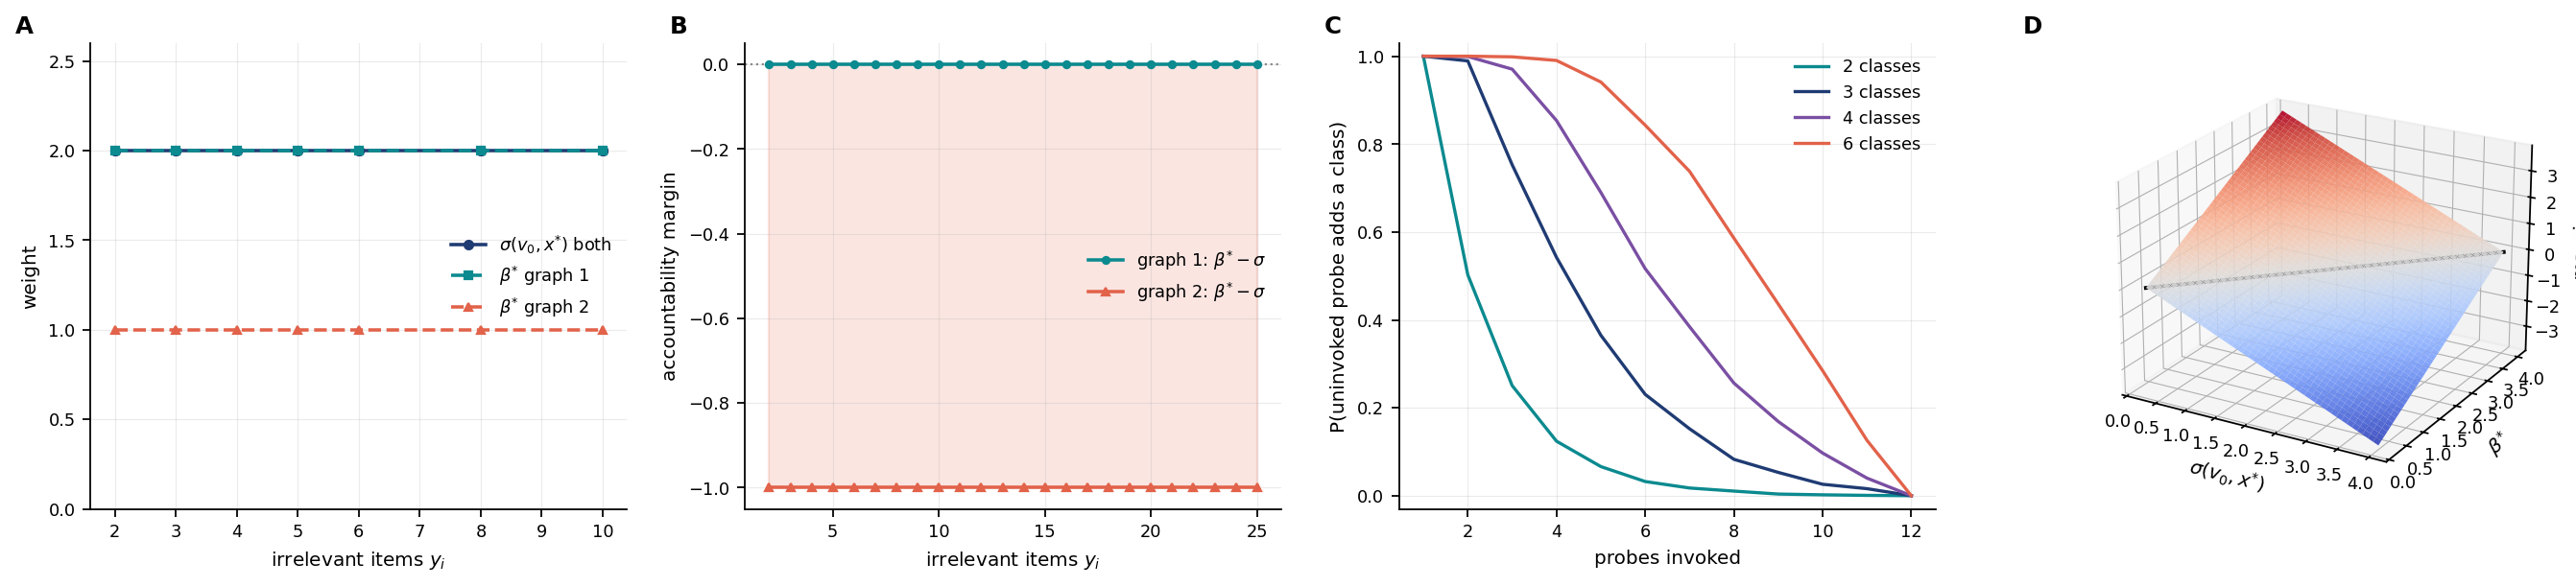
\includegraphics[width=\textwidth]{figures/panel_6_separation.png}
    \caption{\textbf{The Verdict Is a Global Quantity, and the Witness Is
    Invisible to Every Local One.}
    (\textbf{A})~The witness pair of Theorem~\ref{thm:query-separation} as the
    number of irrelevant items $y_i$ grows along the linear $x$-axis ($2$ to
    $10$), weights on the linear $y$-axis. The pair alignment
    $\str(v_0,x^{\star})$ is identical in the two graphs (navy, filled and open
    markers coincident at exactly $2.0$), while the system floors separate:
    $2.0$ in graph~1 (teal) against $1.0$ in graph~2 (crimson). The two graphs
    have identical contact relations at every size---the same assertion set,
    hence identical under every retrieval query---yet the verdicts differ at
    $\eps=0$.
    (\textbf{B})~The accountability margin $\flo^{\ast}-\str(v_0,x^{\star})$ on
    the linear $y$-axis, swept to $25$ irrelevant items on the linear $x$-axis.
    Graph~1 sits at exactly $0$ (accountable, teal) and graph~2 at exactly
    $-1$ (not accountable, crimson), the two shaded to the zero reference and
    both flat: adding items that lie on no path between the queried pair moves
    the verdict without moving anything local to it. This isolates the
    asymmetry of Remark~\ref{rem:separation-meaning}---the queried quantity is
    local and equal, the threshold is global and different. A bounded pattern
    confined to the queried pair's neighbourhood is fooled in $200$ of $200$
    instances (Corollary~\ref{cor:attributed}), and none of $500$
    corpus-determined maps spanning five families separates the two graphs
    (Theorem~\ref{thm:corpus-separation}).
    (\textbf{C})~Probability that an uninvoked probe still reaches a new
    equivalence class, on the linear $y$-axis ($0$ to $1$), versus probes
    already invoked on the linear $x$-axis ($1$ to $12$), for registries
    admitting two, three, four, and six classes, $4000$ draws per point. A
    fixed confidence criterion is satisfied at the first probe while this
    probability remains near unity, and it decays only as the registry is
    exhausted---the content of Theorem~\ref{thm:closure-stronger} (Closure Is
    Strictly Stronger). Over $300$ runs to closure, $169$ terminated in
    convergent closure and $131$ in contested closure, with none running on
    (Theorem~\ref{thm:decline}).
    (\textbf{D})~The verdict surface: the accountability margin as a
    three-dimensional surface (coolwarm) over the pair alignment
    $\str(v_0,x^{\star})$ on the $x$-axis and the system floor $\flo^{\ast}$ on
    the $y$-axis, both $0.2$ to $4.0$, at $\eps=0$, elevation $22^{\circ}$
    azimuth $-60^{\circ}$. The black line is the decision boundary
    $\str=\flo^{\ast}$, above which a determination is accountable and below
    which it is not. The two witness graphs sit on opposite sides of this
    boundary while agreeing on every quantity a store of assertions records;
    the pair decides the verdict correctly on $200$ of $200$ random instances
    and separates the witness that no corpus-determined map separates
    (Theorem~\ref{thm:pair-expresses}).}
    \label{fig:panel6}
\end{figure*}

% =====================================================================
\section{The master equivalence}
\label{sec:master}
% =====================================================================

We close the theory by showing every structure above is the same fact.

\begin{theorem}[Master equivalence]
\label{thm:master}
For a contact graph over a non-completable medium, the following are
equivalent:
\begin{enumerate}[label=\textup{(\roman*)},leftmargin=2.0em,itemsep=1pt]
\item there is an identifiable item---a proper part told from the rest at
positive cost;
\item the floor is positive, $\flo>0$ (\Cref{thm:floor});
\item individuation is by negation without selector (\Cref{thm:negation});
identity is the invariant minimum cut and never a point
(\Cref{thm:invariant,thm:region}); the invariant is not extractable by its
bearer (\Cref{thm:unextractable}); processes are monotone non-returning
residue chains (\Cref{thm:propagator,thm:monotone}); every act of
individuation blunts its instrument (\Cref{thm:blunt}); and the catalogue is
the propagation table at rest (\Cref{thm:catalogue-table});
\item the perfect repeatable traceless instrument---an individuation leaving
no residue and no trace in the instrument---does not exist
(\Cref{thm:no-perfect}).
\end{enumerate}
\end{theorem}

\begin{proof}
$(\mathrm{i})\Rightarrow(\mathrm{ii})$: an identifiable proper part has
positive separation cost by \Cref{thm:floor-derived,thm:floor}.
$(\mathrm{ii})\Rightarrow(\mathrm{iii})$: each listed structure is proved from
$\flo>0$ in the theorem cited.
$(\mathrm{iii})\Rightarrow(\mathrm{iv})$: \Cref{thm:no-perfect} is among the
consequences, being proved from \Cref{thm:floor} and \Cref{thm:monotone}, both
listed.
$(\mathrm{iv})\Rightarrow(\mathrm{i})$: if no traceless instrument exists then
every individuation costs more than zero, i.e.\ some thing is told from the
rest at positive cost---an identifiable item. The cycle closes.
\end{proof}

\begin{remark}[One fact, many faces]
\label{rem:master-reading}
\Cref{thm:master} says the paper has one premise and many restatements of its
consequence. Telling a thing from the rest of a whole that cannot be finished
costs a strictly positive irreducible residue. That residue is at once the
thing's identity (\Cref{thm:region}), the cause of the next determination
(\Cref{thm:propagator}), the trace deposited in the instrument
(\Cref{thm:blunt}), the reason no determination is a point
(\Cref{cor:no-sharp}), and---read at rest versus under process---the reason a
catalogue and a propagation machinery are one object
(\Cref{thm:catalogue-table}).
\end{remark}

% =====================================================================
\part{Architecture, Validation, and Scope}
\label{part:arch}
% =====================================================================

% =====================================================================
\section{The blueprint}
\label{sec:blueprint}
% =====================================================================

We convert the theory into commitments a running system must honour. Each is
stated as a checkable predicate together with the theorem that makes the
predicate the right one. These are design commitments, honourable by
construction, not empirical hypotheses about any existing system.

\begin{binv}[Conserved invariant]
\label{binv:invariant}
The system computes, from its own structure alone, the family of separation
costs $\bigl(\str(v)\bigr)_v$ and their realising cuts, and this family is
preserved under every relabelling of items.\\
\emph{Predicate:} for a random relabelling $\phi$, the multiset
$\set{\str(v)}$ is unchanged and each resting cut maps onto a resting cut.\\
\emph{Certified by:} \Cref{thm:invariant}, \Cref{prop:char}.
\end{binv}

\begin{binv}[Never-resetting record]
\label{binv:record}
Every committed act increments a monotone counter that no operation
decrements, and two states with equal configuration and unequal counters are
distinct states.\\
\emph{Predicate:} no code path decreases the counter; ``undo'' is implemented
as a compensating commit that increments it.\\
\emph{Certified by:} \Cref{thm:monotone}, \Cref{cor:record-time}.
\end{binv}

\begin{binv}[Determination by search, not by lookup]
\label{binv:search}
Every determination is a freshly computed cut against the current graph. No
determination is returned from a cache of prior determinations.\\
\emph{Predicate:} the determination path contains no read of a stored answer;
every answer's provenance is a set of cuts computed at the current record.\\
\emph{Certified by:} \Cref{cor:no-staleness}, \Cref{prop:staleness}.
\end{binv}

\begin{binv}[Deposit on every propagation]
\label{binv:deposit}
Every process-side propagation commits its residue into the graph before its
determination is returned.\\
\emph{Predicate:} the record after a determination strictly exceeds the record
before; the uncommitted capacity of the items involved strictly decreases.\\
\emph{Certified by:} \Cref{thm:blunt}, \Cref{thm:pair-blunts}.
\end{binv}

\begin{binv}[Accretive update]
\label{binv:accretive}
Structural change adds items, contacts, and committed values; no update leaves
a unit open, and no update is implemented as teardown followed by rebuild.\\
\emph{Predicate:} for every unit and every intermediate stage of an update, a
resting cut is attained.\\
\emph{Certified by:} \Cref{thm:termination-crit}, \Cref{cor:accretion},
\Cref{cor:snapshot}.
\end{binv}

\begin{binv}[No system verdict]
\label{binv:no-verdict}
The system reports determinations, classes, and declines; it does not report
success or failure.\\
\emph{Predicate:} the vocabulary exposed to consumers contains no comparison
of an achieved determination to an expected one.\\
\emph{Certified by:} \Cref{thm:no-verdict}, \Cref{thm:receiver},
\Cref{thm:decline}.
\end{binv}

\begin{proposition}[The invariants are independent]
\label{prop:invariants-independent}
No invariant of \Cref{binv:invariant}--\Cref{binv:no-verdict} follows from the
conjunction of the others: for each, there is a system satisfying the
remaining five and violating it.
\end{proposition}

\begin{proof}
For each invariant we exhibit the violating system. Violating
\Cref{binv:invariant}: a system storing labels as identity, which satisfies the
others but fails relabelling-invariance by \Cref{thm:invariant}. Violating
\Cref{binv:record}: a system with a resettable counter, which may still compute
cuts freshly and accrete. Violating \Cref{binv:search}: a system caching
determinations, which may still keep a monotone record. Violating
\Cref{binv:deposit}: a system computing cuts freshly but discarding the
residue, which keeps a record advanced by other means. Violating
\Cref{binv:accretive}: a system that rebuilds on migration but otherwise
behaves correctly. Violating \Cref{binv:no-verdict}: a system that adjudicates
between classes at contested closure while honouring the other five.
\end{proof}

\begin{remark}[What a violation costs]
\label{rem:violation-cost}
The invariants are not stylistic. A system violating \Cref{binv:search}
exhibits \Cref{prop:staleness}; one violating \Cref{binv:deposit} occupies the
position of \Cref{cor:stateless-forbidden}; one violating
\Cref{binv:accretive} silently replaces one individual with another
(\Cref{cor:snapshot}) while appearing to preserve it, since $\Char$ is
unchanged; one violating \Cref{binv:no-verdict} presents contested closure as
a determination, discarding the very information \Cref{thm:decline}(ii)
identifies as valuable.
\end{remark}

% =====================================================================
\section{Algorithms}
\label{sec:algorithms}
% =====================================================================

We state the two procedures the construction requires, with their complexity.

\begin{algorithm}[H]
\caption{Construction to closure}
\label{alg:construct}
\begin{algorithmic}[1]
\Require sources $\mathcal{U}$; constructors $C_1,\dots,C_r$ with $r\ge3$ of
distinct kind
\Ensure induced graph $\Gph_\terms$, or a report of contested closure
\State $\Cell\gets\varnothing$;\quad $\terms\gets$ empty map
\Repeat
  \For{each constructor $C_j$ not yet exhausted}
    \State $\terms_j\gets C_j(\mathcal{U})$
    \State $c\gets$ class of $\terms_j$ under
           endpoint-indistinguishability
    \If{$c\notin\Cell$} \State $\Cell\gets\Cell\cup\set{c}$ \EndIf
  \EndFor
\Until{no constructor adds a class to $\Cell$}
   \Comment{closure, \Cref{def:closure}}
\If{$\abs{\Cell}=1$}
  \State \Return $\Gph_\terms$ built from the single class
     \Comment{\Cref{thm:decline}(i)}
\Else
  \State \Return \textsc{Decline}$(\Cell)$
     \Comment{\Cref{thm:decline}(ii)}
\EndIf
\end{algorithmic}
\end{algorithm}

\begin{proposition}[Construction terminates]
\label{prop:construct-terminates}
\Cref{alg:construct} terminates in finitely many rounds, and its output is
either a single-class graph or a contested-closure report.
\end{proposition}

\begin{proof}
The constructor set is finite and $\Cell$ is a partition of a finite set of
reachable classes, so $\Cell$ can grow only finitely often; once no
constructor adds a class the loop exits. The dichotomy is
\Cref{thm:decline}.
\end{proof}

\begin{algorithm}[H]
\caption{Determination by the directional pair}
\label{alg:determine}
\begin{algorithmic}[1]
\Require graph $\Gph$; seed $v_0$; target $x^{\star}$; probes
$\gamma_1,\dots,\gamma_k$; budget $\att$; tolerance $\eps$
\Ensure accountable class or decline; $\Gph$ advanced
\State $R\gets\seek(x^{\star})$
   \Comment{reachability, $\mathcal{O}(\abs{\V}+\abs{\E})$}
\State $N\gets\nec(R,x^{\star})$
   \Comment{domination, near-linear \citep{lengauer1979}}
\State $\alloc^{\star}\gets$ water-filling over $N$ at price $\price$
   \Comment{\Cref{thm:waterfill}}
\State $\Cell\gets\varnothing$
\Repeat
  \State invoke each $\gamma_i$ with $a_i^{\star}>0$; commit residues into
         $\Gph$ \Comment{\Cref{binv:deposit}}
  \State $\Cell\gets\Cell\cup\set{\text{classes reached}}$
\Until{no uninvoked probe adds a class}
   \Comment{closure, \Cref{def:closure}}
\State $\flo^{\ast}\gets\min_v\str(v)$;\quad
       $s\gets\str(v_0,x^{\star})$
\If{$s\le\flo^{\ast}+\eps\Om$ \textbf{and} $\abs{\Cell}=1$}
  \State \Return the single class \Comment{\Cref{def:accountable}}
\Else
  \State \Return \textsc{Decline}$(\Cell)$
\EndIf
\end{algorithmic}
\end{algorithm}

\begin{theorem}[Determination cost]
\label{thm:determine-cost}
\Cref{alg:determine} performs $\mathcal{O}(\abs{\V})$ minimum-cut
computations, one reachability traversal, one dominator computation, one
convex allocation, and at most $\abs{\Cell}\cdot k$ probe invocations. All
components are exactly computable; no step requires an index over stored
determinations and no step reads a cached answer.
\end{theorem}

\begin{proof}
The system floor requires $\abs{\V}-1$ minimum cuts by
\Cref{def:system-floor}, and the pair alignment one more; each is exact by
maximum flow \citep{fordfulkerson1956,edmondskarp1972,stoer1997}. Reachability
is linear \citep{tarjan1972} and domination near-linear
\citep{lengauer1979}. The allocation is the convex program of
\Cref{thm:waterfill}, solved by bisection on the scalar price. The probe
bound is \Cref{thm:decline}: closure is reached once every probe has been
tried against every reached class. Absence of cached reads is
\Cref{binv:search}.
\end{proof}

\begin{remark}[Where the cost actually sits]
\label{rem:cost-sits}
\Cref{thm:determine-cost} counts graph operations and excludes the cost of
building the graph, exactly as \Cref{rem:comparison-honest} concedes. On a
graph already built, determination is cheap: minimum cuts are polynomial and
the remaining steps are near-linear. The expense is construction, and
\Cref{alg:construct} makes it explicit rather than hiding it in an amortised
training procedure.
\end{remark}


\section{Discussion}
\label{sec:discussion}
% =====================================================================

\subsection{Relation to existing practice}

\paragraph{Knowledge graphs and query languages.}
The construction takes from the knowledge-graph tradition
\citep{hogan2021,smith2007} the idea of a structured medium over which
questions are asked, and departs from it in two places. Nodes are not stored
records: identity is a computed cut (\Cref{thm:region}), which is why the
identifier-stability and cross-reference problems that attend stored
identifiers \citep{wren2008,mcmurry2017} do not arise---there is no identifier
to become stale. Edges are not curated assertions: the causal relation is a
product of a propagation (\Cref{prop:no-edges}). And the query semantics
differ in kind, not degree: \Cref{thm:query-separation} shows admissibility
lies outside the expressive power of conjunctive queries with regular path
expressions \citep{perez2009,angles2017}, for the structural reason that the
verdict depends on a minimum over the entire item set while pattern matching
forms no such minimum.

\paragraph{Retrieval augmentation.}
Retrieval-augmented generation \citep{lewis2020} is, in the vocabulary of
\Cref{sec:probing}, an implementation of $\seek$ alone.
\Cref{cor:no-single} identifies the missing operator and
\Cref{thm:separation-operators} shows it is not obtainable by improving the
retriever. Separately, \Cref{cor:stateless-forbidden} applies to the generating
component regardless of what is retrieved: supplying material to a determiner
does not make the determiner deposit.

\paragraph{Long-context architectures.}
Efficient long-context methods \citep{tay2022,vaswani2017} lower the marginal
cost of carrying more material but do not change what is carried, and the
observed degradation of attention over long inputs \citep{liu2024} is a
symptom of carrying the wrong thing. \Cref{rem:carry-structure} states the
alternative: carry committed structure, which retains the links
(\Cref{thm:three}(ii)), and regenerate material on demand. The two approaches
compose rather than compete.

\paragraph{Hallucination.}
The literature treats confident incorrect output as a quality defect to be
reduced \citep{ji2023,bender2021}. \Cref{thm:closure-stronger} locates a
structural cause: a determiner stopping on confidence halts at the first
internally-consistent cluster it reaches, and no amount of calibration
converts a confidence threshold into a closure test, because closure quantifies
over probes not yet invoked. \Cref{thm:decline} supplies the alternative
terminal state.

\paragraph{Provenance and reproducibility.}
The relocation of reproducibility from results to protocol
(\Cref{rem:repro}) is the provenance stance \citep{moreau2013,davidson2008}
made structural: by \Cref{cor:repeat} repeated determinations need not agree,
so what must be recorded is the protocol and the committed structure, not the
determination. This aligns the computational case with the experimental one
\citep{peng2011,sandve2013,openscience2015}.

\paragraph{Actor and dataflow models.}
Probes reading and committing over a shared medium resemble actor and dataflow
models \citep{hewitt1973,kahn1974,lee1995}, and the monotone record is a
logical clock \citep{lamport1978}. The departure is that the dependency
structure is not declared: by \Cref{prop:no-edges} the causal edge set is
induced by a propagation rather than given to a scheduler.

\subsection{What the development assumes and does not supply}

The one input the calculus does not derive is the term map
(\Cref{def:term-map}): which distinctions each source draws. Everything
downstream is forced---given the graph, the floor, the invariant, the record,
the table, the directional identity, the allocation, and the separation are
all theorems (\Cref{thm:tau-agnostic}). The term map is a modelling choice
whose quality bounds the resolution of the result but never its soundness
(\Cref{cor:coarsen}), and whose quality is measurable without ground truth
(\Cref{cor:quality-signal}). Sharpening it is the natural axis of further
work, and is the single point at which a learned component enters, bounded to
the task of drawing distinctions.

One further premise is environmental rather than structural:
\Cref{ax:concave}, the concavity of gain profiles, on which
\Cref{thm:waterfill} alone depends. Where it fails, the discrete selection of
\Cref{thm:knapsack} governs instead. We flag the dependence because it is the
only place in the paper where a result rests on a claim about the problem
rather than about the structure.

\subsection{Honest limitations}

\begin{enumerate}[leftmargin=1.6em,itemsep=2.5pt]
\item \textbf{Construction cost is excluded.} Every complexity figure counts
graph operations on a graph already built
(\Cref{rem:cost-sits},\Cref{rem:comparison-honest}). A corpus-determined map
amortises its construction over all later queries; the present construction
pays per source read. This is a real asymmetry and the honest comparison is
not that one dominates but that they answer different questions.

\item \textbf{The self-verification result is conditional.}
\Cref{thm:self-diagonal} is exactly as strong as its closure hypothesis
(\Cref{rem:two-arguments}). The unconditional result is
\Cref{thm:unextractable}, which is weaker: it says the invariant is not
extractable as a value, not that self-verification is directly contradictory.

\item \textbf{Necessity is domination, not reachability, and seeds are
separate.} \Cref{prop:nec-subset} gives only the inclusion, and
\Cref{thm:separation-operators}(iii) exhibits its strictness. The exact
criterion is \Cref{prop:domination}, stated for non-seed items; seeds are
load-bearing by definition and must be handled apart
(\Cref{rem:contribution-care}). A system computing reachability and calling it
necessity over-retains, and one that mismeasures the contribution collapses
the two operators entirely.

\item \textbf{The floor readout is monotone, not calibrated.}
\Cref{rem:quality-honest} states this, and \Cref{fig:panel4}C makes it
concrete: the degenerate family of term maps---every source drawing identical
distinctions---induces among the highest realised floors while discriminating
worst. A rising floor indicates refinement is occurring; a high floor is not
by itself evidence of a good term map, and optimising it directly would be an
error.

\item \textbf{Two premises, and where they fail.} \Cref{ax:finite} and
\Cref{ax:noncompletable} hold for essentially every realised system with
bounded memory and an open-ended task. Where an agent is effectively unbounded
or its medium is genuinely completable---a closed finite world it can
exhaust---the floor may vanish, residues can reach zero, determinations become
points, and the development is not compelled. In that degenerate regime a
stateless determiner is not occupying a forbidden position, because the
forbidden position exists only when $\flo>0$. The interest of the account is
exactly that realised systems are not in that regime.
\end{enumerate}

\subsection{The picture in one statement}

Telling a thing from the rest of a whole that cannot be finished costs a
strictly positive, irreducible residue, and deposits it into the instrument as
much as into the sample. An instrument that claims otherwise claims a position
the floor forbids. What exists instead is a single table: read at rest, it is a
catalogue of invariant cells; read under process, it returns cells of the same
kind that rest cannot produce. The residue of each process flows back into the
catalogue as committed structure, which is where the instrument blunts, and
which is why the catalogue is the process's identity. An individual is that
catalogue's conserved cut structure together with its unrepealable record:
parts may be wholly replaced without touching it, provided nothing is ever left
unterminated; reconstruction to identical specification yields a new
individual; and no structure can verify its own identity, so identity is what
consuming systems individuate it as, and they may correctly disagree.

% =====================================================================
\section{Conclusion}
\label{sec:conclusion}
% =====================================================================

We set out to describe a pairing of a generative determiner with a structured
medium, and found that the pairing is not a composition of two systems.

From a single premise---that the whole against which anything is distinguished
cannot be finished---we derived a strictly positive floor on the cost of every
act of individuation (\Cref{thm:floor}), and then the fact that gives the floor
its force: individuation is symmetric, depositing its residue into the
instrument exactly as into the sample (\Cref{thm:symmetry},
\Cref{thm:blunt}). The perfect repeatable traceless instrument is the object
the floor excludes (\Cref{thm:no-perfect}), and a determiner that is unchanged
by determining asserts it is that object
(\Cref{cor:stateless-forbidden}). Its two visible symptoms---answering as a
state it has left (\Cref{prop:staleness}), and converting its own prior
propagation into content whose causal links are gone
(\Cref{prop:reification})---are consequences, not incidental defects.

The remedy is a direction rather than a component. The causal propagation table
evaluated at the trivial process is a catalogue of resting cells, and evaluated
at a nontrivial process returns objects of the same type computed under
propagation (\Cref{thm:catalogue-table}). A structured medium and a generative
determiner are therefore one map at two settings of its process argument
(\Cref{cor:one-object}), and the residue of every process-side propagation is
committed into the medium (\Cref{thm:pair-blunts}), which is where the
instrument blunts and which is the precise sense in which the medium is the
determiner's identity (\Cref{cor:graph-is-identity}). The pair then has neither
symptom: nothing is re-presented (\Cref{cor:no-representation}) and nothing is
stale (\Cref{cor:no-staleness}), and repeated determinations correctly need not
agree (\Cref{cor:repeat}).

Identity itself turned out to require a pair: the conserved, non-local,
relabelling-invariant cut structure together with the unrepealable record
(\Cref{def:individual}). The operative criterion is continuity of termination
rather than continuity of parts (\Cref{thm:termination-crit}), which
adjudicates gradual replacement, reconstruction, and copying, and yields two
engineering commitments---no snapshot-restore, accretive migration only
(\Cref{cor:snapshot}, \Cref{cor:accretion}). No structure verifies its own
identity (\Cref{thm:unextractable}, \Cref{thm:self-diagonal}), so identity is
consumer-relative (\Cref{thm:receiver}) and the system issues no verdict
(\Cref{thm:no-verdict}).

As a working architecture the pair takes one declared input---the term map---%
and is correct for any value of it (\Cref{thm:tau-agnostic}), so a fallible
constructor coarsens resolution without corrupting soundness
(\Cref{cor:coarsen}) and its quality is readable from the realised floor
without ground truth (\Cref{cor:quality-signal}). Probes over the medium
compose multiplicatively rather than by vote (\Cref{thm:multiplicative}),
require no fewer than three mutually supporting members
(\Cref{thm:triangle}), divide a finite budget by water-filling at a single
shadow price (\Cref{thm:waterfill}), and must be paired with a distinct pruning
operator that no single mechanism supplies
(\Cref{thm:separation-operators}). Determination stops on closure, which is
strictly stronger than any confidence threshold
(\Cref{thm:closure-stronger}), and reports contested closure as a first-class
outcome rather than resolving it (\Cref{thm:decline}).

Finally, the pair answers a class of question that no store of local content
can express. Accountability is a global minimum over the item set stated in
local terms, and the verdict is therefore invisible to pattern matching over
assertions (\Cref{thm:query-separation}), to attributed assertions
(\Cref{cor:attributed}), and to any map determined by a finite corpus
(\Cref{thm:corpus-separation}). The quantity is polynomial-time computable and
inexpressible, which is an unusual combination and the reason the gap has
persisted (\Cref{cor:separation-stated}).

The construction cost is real and we have not hidden it: building the medium is
work that a corpus-determined map amortises and this one pays per source. What
is bought is a determiner that has an identity, that cannot be stale, that
deposits what it learns into the structure it reasons over, that knows when it
has not resolved, and that can say so.

% =====================================================================
\bibliographystyle{plainnat}
\bibliography{references}
% =====================================================================

\end{document}
